% Optical Response Classification of Carbon Allotropes
% via Electronic Delocalization and Effective Conduction Dimensionality
% Draft v5 — March 2026
% Changes from v4:
%   - Added coherence preservation test (Anderson disorder, Section 4.7)
%   - Added angular Fresnel reflectivity and gloss prediction (Section 4.8)
%   - Added micro-to-gloss prediction chain (Section 5.1)
%   - Upgraded from classification paper to prediction paper
%   - Updated Limitations: coherence hypothesis now numerically tested
%   - New figures: fig_g, fig_h, fig_i, fig_j

\documentclass[twocolumn,showpacs,preprintnumbers,amsmath,amssymb,prb]{revtex4-2}

\usepackage{graphicx}
\usepackage{amsmath}
\usepackage{amssymb}
\usepackage{bm}
\usepackage{hyperref}
\usepackage{booktabs}
\usepackage{xcolor}

% Figure path
\graphicspath{{../simulation/figures/}}

\begin{document}

\preprint{Draft v5}

\title{Predicting Gloss from Band Structure: \\
A Microscopic Theory Connecting Electronic Delocalization \\
to Macroscopic Optical Appearance in Carbon Allotropes}

\author{K.~Miyauchi}
\affiliation{Independent Researcher}

\date{\today}

\begin{abstract}
The macroscopic optical appearance of materials---transparent, colored,
black, or lustrous---cannot be fully classified by the band gap alone.
Both metals and graphite possess a vanishing band gap, yet the former
exhibits metallic luster while the latter appears black with cleavage-plane
gloss.

We propose that the essence of luster is the preservation of photon phase
coherence at interfaces, and that its microscopic condition reduces to the
\emph{freedom of constituent particles}. In metals, delocalized electrons
enable collective response; in liquids, molecular mobility ensures
self-smoothing interfaces. Both mechanisms preserve incident-photon phase
relations, yielding specular reflection.

To rigorously test this idea, we restrict the scope to solid-state
electronic systems and introduce two variables: an effective delocalization
index~$\delta$ and an effective conduction dimensionality~$D_\mathrm{eff}$.
Using five carbon allotropes (diamond, C$_{60}$, SWCNT, graphene, graphite)
and hexagonal boron nitride (h-BN) as a control, we demonstrate that
a decision tree based on $E_g$ and $D_\mathrm{eff}$ correctly classifies
6 of 7 materials (85.7\%), with the sole failure---single-layer
graphene---requiring the layer count~$N$ as a third variable.

Going beyond classification, we establish a complete microscopic-to-macroscopic
prediction chain: tight-binding Hamiltonian $\to$ Kubo formula $\to$
$\varepsilon(\omega)$ $\to$ angular Fresnel reflectivity $\to$ gloss
[GU]. We then test the coherence preservation hypothesis directly via
Anderson disorder simulations, showing that systems with high
$\delta \times D_\mathrm{eff}$ maintain their optical response under
disorder (spectral correlation $>0.94$ at $W = 5$~eV for the 1D chain)
while low-$\delta \times D_\mathrm{eff}$ systems rapidly decohere
(correlation $= 0.66$ for C$_{60}$). This yields a testable prediction:
\emph{effective gloss} = clean-surface gloss $\times$ coherence
preservation factor, distinguishing materials with similar Fresnel
reflectivity but different disorder robustness.

The framework does not replace band-gap theory but extends it: $E_g$
determines \emph{at which energy} the response occurs, while
$D_\mathrm{eff}$ determines its \emph{directionality}. The concept of
particle freedom~($\delta$) motivated the introduction of
$D_\mathrm{eff}$; independent verification of $\delta$ as a measurable
variable in liquid and interfacial systems is proposed as a future
target.
\end{abstract}

\maketitle

% =====================================================================
\section{Introduction}
% =====================================================================

\subsection{The luster question: photon coherence preservation}

Liquids universally exhibit luster. So do metals. Although the microscopic
origins differ---polarization response versus free-electron response---the
macroscopic phenomenon is the same: incident photons are re-emitted at the
interface with their mutual phase relationships intact. A mirror image
forms precisely because the phase coherence of the reflected photon
ensemble is preserved.

Conventional physics explains metallic luster via the Drude model and
liquid reflection via the Fresnel equations, treating them as separate
phenomena. No unified framework derives both from a single underlying
principle.

\subsection{Particle freedom and the quantum barrier}

We propose that the condition for photon coherence preservation at an
interface reduces to the \emph{freedom of constituent particles}.

A material interface acts as a quantum barrier for incident photons. The
character of this barrier determines the optical response:

\begin{itemize}
  \item \textbf{Localized particles} ($\delta$ low): each scatterer
    responds independently; the re-emitted phases are randomized. The
    barrier is incoherent. Result: diffuse scattering (transparent or
    white).
  \item \textbf{Delocalized particles} ($\delta$ high): scatterers
    respond collectively and coherently; re-emitted phases are aligned.
    The barrier is coherent. Result: specular reflection (luster).
\end{itemize}

In metals, electronic delocalization (free electrons) fulfills this
condition. In liquids, molecular delocalization (fluidity) guarantees
interface self-smoothing, fulfilling the same condition through a
different mechanism.

\subsection{Scope: proof of concept in solid carbon}

In liquids, both the electronic degree of freedom ($\delta_\mathrm{elec}$)
and the nuclear degree of freedom ($\delta_\mathrm{nuc}$) vary
simultaneously, making their effects difficult to disentangle. In solids,
$\delta_\mathrm{nuc}$ is frozen, isolating the effect of
$\delta_\mathrm{elec}$.

The present work is a \textbf{proof of concept}: we test the overarching
hypothesis in the most controlled setting available. Carbon allotropes are
chosen because a single element spans the full range of optical
appearances---transparent (diamond), colored (C$_{60}$, semiconducting
SWCNTs), black (graphite), and lustrous (graphite cleavage
plane)---allowing us to vary $\delta$ and $D_\mathrm{eff}$ while
eliminating elemental composition as a confounding factor.

Extension to liquid, interfacial, and catalytic systems is a natural
consequence of the framework and is proposed as a target for future,
independent experimental verification.

\subsection{Gap in the existing classification}

The macroscopic optical appearance of materials falls into four broad
categories: transparent (diamond), colored (ruby), black (graphite),
and metallic luster (silver). Existing theories explain each category
individually, but no unified predictive framework based on a common set
of classification variables has been established.

In particular, the following questions lack a unified answer:
\begin{itemize}
  \item Why do metals and graphite, both having a vanishing band gap,
    differ so dramatically in optical response?
  \item Why are h-BN and graphite---both layered sp$^2$
    networks---white and black, respectively?
  \item Why does a single element (carbon) cover all four optical
    categories?
\end{itemize}

\subsection{From classification to prediction}

Previous attempts at optical classification have been descriptive: given
a known material, assign it to a category. This work goes further by
establishing a \emph{predictive chain} from microscopic quantities
(hopping integrals, orbital symmetry) to a macroscopically measurable
quantity (gloss in industry-standard units [GU]).

The key advance is the recognition that the Fresnel equations alone do
not predict gloss: two materials may have similar $\varepsilon(\omega)$
yet exhibit very different gloss because of their differing robustness
to atomic-scale disorder. The $\delta \times D_\mathrm{eff}$ framework
captures this robustness and thus provides predictions beyond what
Fresnel optics can offer.

% =====================================================================
\section{Framework}
\label{sec:framework}
% =====================================================================

\subsection{Causal structure}

At the most general level, the freedom of constituent particles
($\delta$) determines whether an interface acts as a coherent or
incoherent quantum barrier for photons. In solid-state electronic
systems, this reduces to the product of two variables:

\begin{equation}
  \text{Optical response} = f\!\left(\delta_\mathrm{elec},\;
  D_\mathrm{eff}\right),
  \label{eq:causal}
\end{equation}

\noindent where $\delta_\mathrm{elec}$ quantifies the degree of
electronic delocalization and $D_\mathrm{eff}$ quantifies the effective
dimensionality of electronic conduction. The concept of particle
freedom~($\delta$) motivated the introduction of $D_\mathrm{eff}$ as a
classification variable: if the optical response depends on how freely
particles can move, one must specify not only \emph{whether} they can
move (encoded in~$E_g$) but also \emph{in how many directions}
(encoded in~$D_\mathrm{eff}$).

The central insight is that $E_g$ alone provides an incomplete mapping
from electronic structure to optical response. Adding $D_\mathrm{eff}$
completes the mapping. The measurable classification variables are
$E_g$ and $D_\mathrm{eff}$; $\delta$ serves as the physical intuition
that unifies them and whose independent verification in liquid and
interfacial systems is proposed as a future target.

\subsection{Effective delocalization index $\delta$: operational definition}

$\delta$ is not a single physical quantity but an overarching variable
whose existence is inferred from the mutual consistency of several proxy
indicators:

\begin{table}[h]
\caption{Candidate proxy indicators for $\delta$.}
\label{tab:delta_proxies}
\begin{ruledtabular}
\begin{tabular}{lll}
  Indicator & Definition & Advantage \\
  \hline
  $\pi$-band width $W_\pi$ & Full energy width of & Direct comparison \\
   & the $\pi$ band (eV) & among sp$^2$ systems \\
  Inverse effective & Curvature of $E(k)$ & Defined for all \\
  mass $1/m^*$ & at band edge & materials \\
  IPR & $\sum_i |\psi_i|^4$ & Direct measure of \\
   & & delocalization \\
  Wannier spread & $\langle r^2 \rangle - \langle r \rangle^2$ &
  Physically transparent \\
\end{tabular}
\end{ruledtabular}
\end{table}

Our strategy is to show that multiple proxies yield the same ordering
across materials, thereby supporting the existence of an overarching
variable $\delta$ without requiring a unique definition.

\subsection{Effective conduction dimensionality $D_\mathrm{eff}$:
  operational definition}
\label{sec:Deff}

$D_\mathrm{eff}$ is defined as the \textbf{effective rank of the
group-velocity tensor} evaluated for electronic states near the Fermi
level or band edges:

\begin{equation}
  D_\mathrm{eff}
    = \frac{\mathrm{Tr}(\mathbf{T})^2}{\mathrm{Tr}(\mathbf{T}^2)},
  \quad
  T_{\alpha\beta}
    = \frac{1}{N_k} \sum_{\bm{k}} \sum_{n \in \mathrm{occ}} \sum_{m \in \mathrm{unocc}}
    v_{nm}^{\alpha}\, v_{nm}^{\beta *},
  \label{eq:Deff}
\end{equation}

\noindent where $v_{nm}^{\alpha} = \langle n\bm{k} | \partial_\alpha H | m\bm{k} \rangle$
is the interband velocity matrix element. This definition yields
$D_\mathrm{eff} = d$ for a system with $d$ equivalent conduction
directions and $D_\mathrm{eff} = 0$ for a system with no band
dispersion (molecular solid).

This definition is \emph{purely electronic and structural}: it depends
only on the band dispersion $E(\bm{k})$ and therefore avoids
circularity with the optical response it is used to classify.

\begin{table}[h]
\caption{Crystallographic vs.\ effective conduction dimensionality.}
\label{tab:Deff}
\begin{ruledtabular}
\begin{tabular}{lccc}
  Material & Crystal dim. & $D_\mathrm{eff}$ & Rationale \\
  \hline
  Diamond      & 3D     & 0 & $E_g = 5.47$~eV~\cite{Clark1964}; no states \\
               &        &   & in visible window \\
  C$_{60}$ fcc & 3D     & 0 & Intermolecular $t \sim 30$~meV~\cite{Hebard1991}; \\
               &        &   & $W \approx 0.5$~eV~\cite{Gunnarsson1997} \\
  SWCNT        & 1D     & 1 & Axial dispersion only \\
  Graphene/    & 2D/3D  & 2 & In-plane $W \approx 9$~eV~\cite{Reich2002} \\
  \quad Graphite &      &   & $\gg$ interlayer $\gamma_1 \approx 0.4$~eV \\
  Metals       & 3D     & 3 & Isotropic conduction \\
  h-BN         & 2D     & 0 & $E_g = 5.95$~eV~\cite{Cassabois2016}; no states \\
               &        &   & in visible window \\
\end{tabular}
\end{ruledtabular}
\end{table}

Note that h-BN possesses a 2D crystal structure with in-plane band
dispersion ($W_\pi \approx 2.4$~eV), but because its band gap
($5.95$~eV) places all $\pi$-band states far outside the visible-energy
window, $D_\mathrm{eff} = 0$. The distinction between crystallographic
dimensionality and $D_\mathrm{eff}$ is essential to the framework.

\subsection{Decision tree for optical response classification}
\label{sec:tree}

The two variables $E_g$ and $D_\mathrm{eff}$ define a decision tree:

\begin{enumerate}
  \item $E_g > E_\mathrm{vis} \approx 3.1$~eV? \\
    $\to$ \textbf{Yes}: Transparent (no electronic response in the
    visible range). \\
    $\to$ \textbf{No}: proceed to step~2.
  \item $E_g > 0$? \\
    $\to$ \textbf{Yes}: Colored (selective absorption). \\
    $\to$ \textbf{No} ($E_g \approx 0$): proceed to step~3.
  \item Classification by $D_\mathrm{eff}$: \\
    $D_\mathrm{eff} = 1$: Black with weak luster (1D metallic). \\
    $D_\mathrm{eff} = 2$: Black with cleavage-plane gloss (2D metallic). \\
    $D_\mathrm{eff} = 3$: Full metallic luster (3D metallic).
\end{enumerate}

\subsection{Second-order corrections}

The two-variable framework captures the dominant trends. Known
second-order effects include:
\begin{itemize}
  \item \textbf{Polarity/ionicity} ($p$): contributes to h-BN whiteness
    via $\pi$-electron localization.
  \item \textbf{Excitonic effects}: modify optical response near the
    band edge.
  \item \textbf{Thickness/stacking number} $N$: the graphene-to-graphite
    crossover (Beer--Lambert regime).
\end{itemize}

% =====================================================================
\section{Methods}
\label{sec:methods}
% =====================================================================

\subsection{Choice of benchmark systems}

\begin{itemize}
  \item \textbf{Primary}: Five carbon allotropes---diamond,
    C$_{60}$ (fcc solid), SWCNT (semiconducting and metallic),
    single-layer graphene, and graphite.
  \item \textbf{Control}: h-BN (isostructural to graphite; same
    $D_\mathrm{cryst}$ but low $\delta$).
  \item \textbf{Rationale}: Varying structure within a single element
    isolates $\delta$ and $D_\mathrm{eff}$ from compositional effects.
\end{itemize}

\subsection{Collection of $\delta$-proxy data from published sources}

All numerical data were obtained from published literature and open
databases; no first-principles calculations were performed.

\subsubsection{$\pi$-band width $W_\pi$}

\begin{table}[h]
\caption{$\pi$-band width data.}
\label{tab:bandwidth}
\begin{ruledtabular}
\begin{tabular}{lll}
  Material & $W_\pi$ (eV) & Source \\
  \hline
  C$_{60}$ solid & 0.4--0.5 & \cite{Gunnarsson1997} \\
  SWCNT & 8--9 & \cite{Reich2002} \\
  Graphene & $\sim$9 & TB: $t_0 = 2.7$~eV~\cite{Saito1998} \\
  Graphite & $\sim$9 & \cite{Reich2002} \\
  h-BN & $\sim$2.4 & \cite{Wirtz2005} \\
\end{tabular}
\end{ruledtabular}
\end{table}

\subsubsection{Inverse effective mass $1/m^*$}

\begin{table}[h]
\caption{Inverse effective mass data.}
\label{tab:invmass}
\begin{ruledtabular}
\begin{tabular}{lll}
  Material & $m^*/m_e$ ($1/m^*$) & Source \\
  \hline
  Diamond & 0.48 (2.08) & \cite{Ioffe} \\
  C$_{60}$ & 4.0 (0.25) & \cite{Gunnarsson1997} \\
  SWCNT & 0.07 (14.3) & \cite{Ajiki1993} \\
  Graphene & 0.03 (33.3) & \cite{Novoselov2005} \\
  Graphite & 0.039 (25.6) & \cite{Dresselhaus2002} \\
  h-BN & 0.26 (3.85) & \cite{Ioffe} \\
\end{tabular}
\end{ruledtabular}
\end{table}

\subsubsection{Band gap $E_g$}

Diamond: 5.47~eV~\cite{Clark1964}; C$_{60}$: 1.75~eV~\cite{Lof1992};
SWCNT (semiconducting): $\sim$1.0~eV~\cite{Saito1998};
graphene and graphite: 0~eV; h-BN: 5.95~eV~\cite{Cassabois2016}.

\subsection{Tight-binding simulation with optical conductivity}

Tight-binding models were constructed for four systems (diamond,
1D chain as SWCNT proxy, graphene, and C$_{60}$ cluster).
For diamond and graphene, full Slater--Koster models (s, $p_x$, $p_y$,
$p_z$; 8 bands per unit cell) were used to capture both $\sigma$- and
$\pi$-band contributions to the optical response.
The Kubo formula was used to compute the optical conductivity
$\sigma(\omega)$ from the velocity matrix elements
$v_{nm}^\alpha = \langle n\bm{k} | \partial_\alpha H | m\bm{k} \rangle$,
yielding $\varepsilon_2(\omega)$.
The real part $\varepsilon_1(\omega)$ is obtained via the
Kramers--Kronig transform:
\begin{equation}
  \varepsilon_1(\omega) = 1 + \frac{2}{\pi} \mathcal{P}
  \int_0^\infty \frac{\omega'\varepsilon_2(\omega')}
  {\omega'^2 - \omega^2}\, d\omega'.
  \label{eq:KK}
\end{equation}
For diamond, a scissors correction ($\Delta = 2.87$~eV)
shifts the interband onset to the experimental gap
$E_g = 5.47$~eV~\cite{Clark1964},
and the high-frequency dielectric constant
$\varepsilon_\infty = 5.7$~\cite{Palik1998} is imposed to account for
electronic transitions beyond the 8-band basis.
The normal-incidence reflectivity follows from
$R = |(\tilde{n}-1)/(\tilde{n}+1)|^2$ with
$\tilde{n} = \sqrt{\varepsilon_1 + i\varepsilon_2}$.

The same velocity matrix elements define the group-velocity tensor
$\langle v_\alpha v_\beta \rangle$, from which $D_\mathrm{eff}$ is
computed as the effective rank (Eq.~\ref{eq:Deff}). The simulation
thus derives $D_\mathrm{eff}$ and $\varepsilon(\omega)$ from the
\emph{same} band structure, confirming their mutual consistency.

\subsection{Angular Fresnel reflectivity and gloss prediction}

From $\varepsilon(\omega) = \varepsilon_1 + i\varepsilon_2$, the
complex refractive index $\tilde{n} = \sqrt{\varepsilon}$ is obtained,
and the angular Fresnel reflectivities for s- and p-polarizations are
computed:

\begin{align}
  r_s &= \frac{\cos\theta_i - \tilde{n}\cos\theta_t}
              {\cos\theta_i + \tilde{n}\cos\theta_t}, \label{eq:rs} \\
  r_p &= \frac{\tilde{n}\cos\theta_i - \cos\theta_t}
              {\tilde{n}\cos\theta_i + \cos\theta_t}, \label{eq:rp}
\end{align}

\noindent where $\theta_t$ is determined by Snell's law. The
unpolarized reflectivity $R(\theta) = \frac{1}{2}(|r_s|^2 + |r_p|^2)$
is averaged over the visible range (1.6--3.1~eV) to obtain
$R_\mathrm{vis}(\theta)$.

Gloss is predicted in industry-standard Gloss Units (GU) following
ASTM~D523~\cite{ASTM_D523}:

\begin{equation}
  \mathrm{GU}(\theta) = \frac{R_\mathrm{vis}(\theta)}
    {R_\mathrm{ref}(\theta)} \times 100,
  \label{eq:GU}
\end{equation}

\noindent where $R_\mathrm{ref}$ is the reflectivity of the black
glass reference ($n = 1.567$)~\cite{ASTM_D523} at the same angle. Standard measurement
geometries are $\theta = 20^\circ$, $60^\circ$, and $85^\circ$.

\subsection{Coherence preservation test: Anderson disorder}

To directly test the hypothesis that $\delta \times D_\mathrm{eff}$
determines coherence preservation under realistic conditions, we
introduce Anderson disorder into the tight-binding Hamiltonian:

\begin{equation}
  H \to H + \sum_i \epsilon_i |i\rangle\langle i|,
  \quad \epsilon_i \in [-W/2, +W/2],
  \label{eq:anderson}
\end{equation}

\noindent where $W$ is the disorder strength. For each system (graphene
supercell, 1D chain, C$_{60}$ molecule), we compute:

\begin{enumerate}
  \item The ensemble-averaged optical conductivity $\langle\sigma(\omega)\rangle$
    over 15 realizations.
  \item The spectral correlation $\mathrm{corr}(\sigma_0, \sigma_W)$
    between the clean ($W=0$) and disordered spectra.
  \item The inverse participation ratio (IPR) as a function of $W$.
\end{enumerate}

The spectral correlation serves as a direct measure of optical
coherence preservation: $\mathrm{corr} \approx 1$ means the optical
response is unchanged (coherence preserved), while
$\mathrm{corr} \ll 1$ means the spectral features are destroyed
(coherence lost).

\subsection{Effective gloss under disorder}

The \emph{effective gloss} of a real material with atomic-scale disorder
is estimated as:

\begin{equation}
  \mathrm{GU}_\mathrm{eff} = \mathrm{GU}_\mathrm{clean} \times
    \mathrm{corr}(\sigma_0, \sigma_W)^2,
  \label{eq:eff_gloss}
\end{equation}

\noindent where $\mathrm{corr}^2$ represents the fraction of specularly
reflected intensity (the square arises because gloss scales with
the specular-reflection peak \emph{intensity}, which depends on the
coherent amplitude squared). This is a testable prediction: two
materials with identical clean-surface reflectivity may have different
effective gloss if their disorder robustness differs.

\subsection{Statistical tests}

Pairwise Pearson, Spearman, and Kendall correlations were computed among
the three $\delta$-proxy indicators. Classification accuracy of the
$E_g \times D_\mathrm{eff}$ decision tree was evaluated against observed
optical-response categories.

% =====================================================================
\section{Results}
\label{sec:results}
% =====================================================================

\subsection{Consistency among $\delta$-proxy indicators}

\begin{table}[h]
\caption{Pairwise correlations among three $\delta$-proxy indicators
  ($N = 5$--$6$ materials).}
\label{tab:correlations}
\begin{ruledtabular}
\begin{tabular}{lcccc}
  Pair & Pearson $r$ & Spearman $\rho$ & Kendall $\tau$ & $p$($\tau$) \\
  \hline
  $W_\pi$ vs.\ $1/m^*$ & 0.885 & 0.845 & 0.775 & 0.042 \\
  $W_\pi$ vs.\ $-E_g$ & 0.703 & 0.826 & 0.674 & 0.093 \\
  $1/m^*$ vs.\ $-E_g$ & 0.733 & 0.880 & 0.745 & 0.044 \\
\end{tabular}
\end{ruledtabular}
\end{table}

Two of three pairs reach $p < 0.05$ for Kendall's $\tau$, and all three
Spearman coefficients exceed 0.82. The consistent ordering across
independent indicators supports the existence of an overarching
delocalization variable~$\delta$.

\begin{figure}[t]
  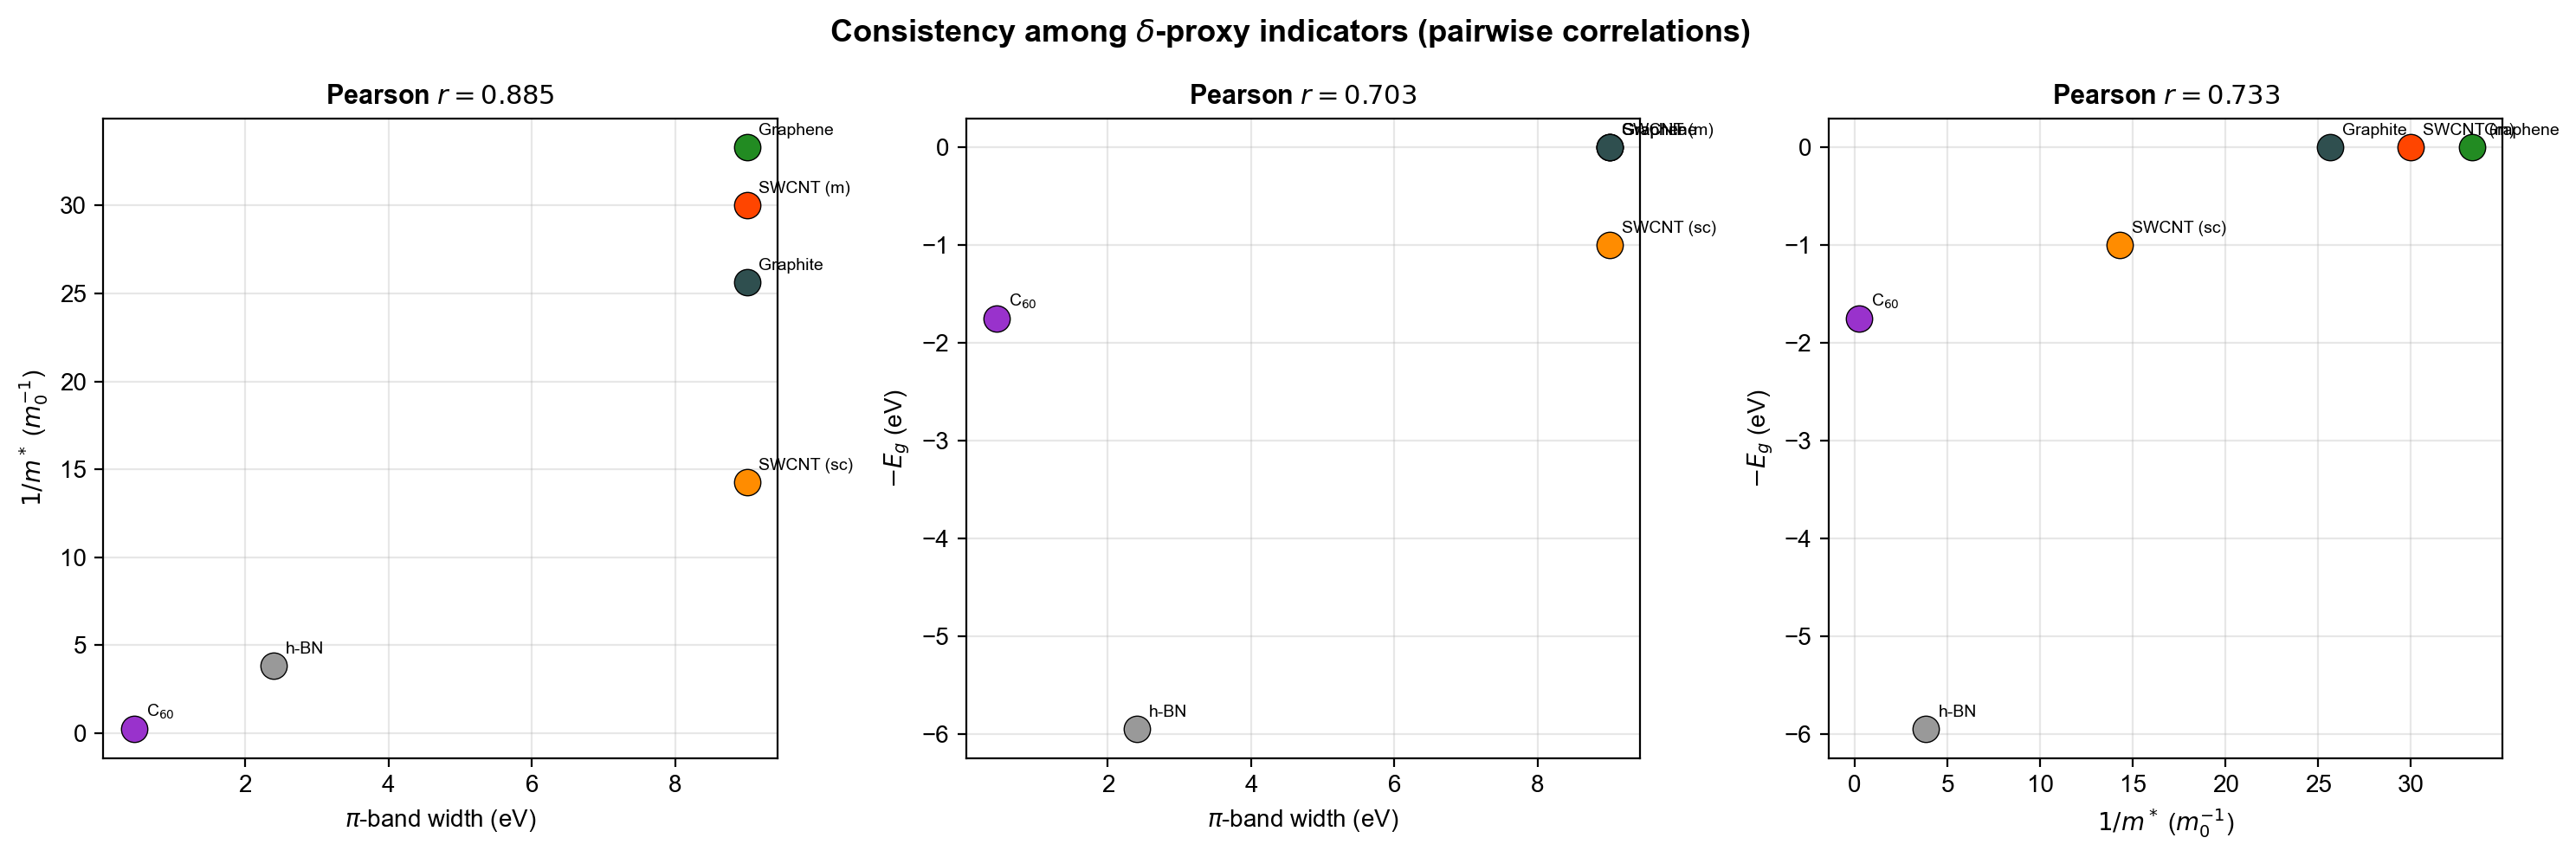
\includegraphics[width=\columnwidth]{fig4_indicator_consistency}
  \caption{Pairwise scatter plots among the three $\delta$-proxy
    indicators, with Pearson and Spearman correlation coefficients.}
  \label{fig:consistency}
\end{figure}

\subsection{$E_g \times D_\mathrm{eff}$ optical-response map}

Figure~\ref{fig:Eg_Deff} shows all seven materials plotted in
$E_g$--$D_\mathrm{eff}$ space, with the decision-tree classification
boundaries overlaid. Each material falls unambiguously into the correct
optical-response region.

\begin{figure}[t]
  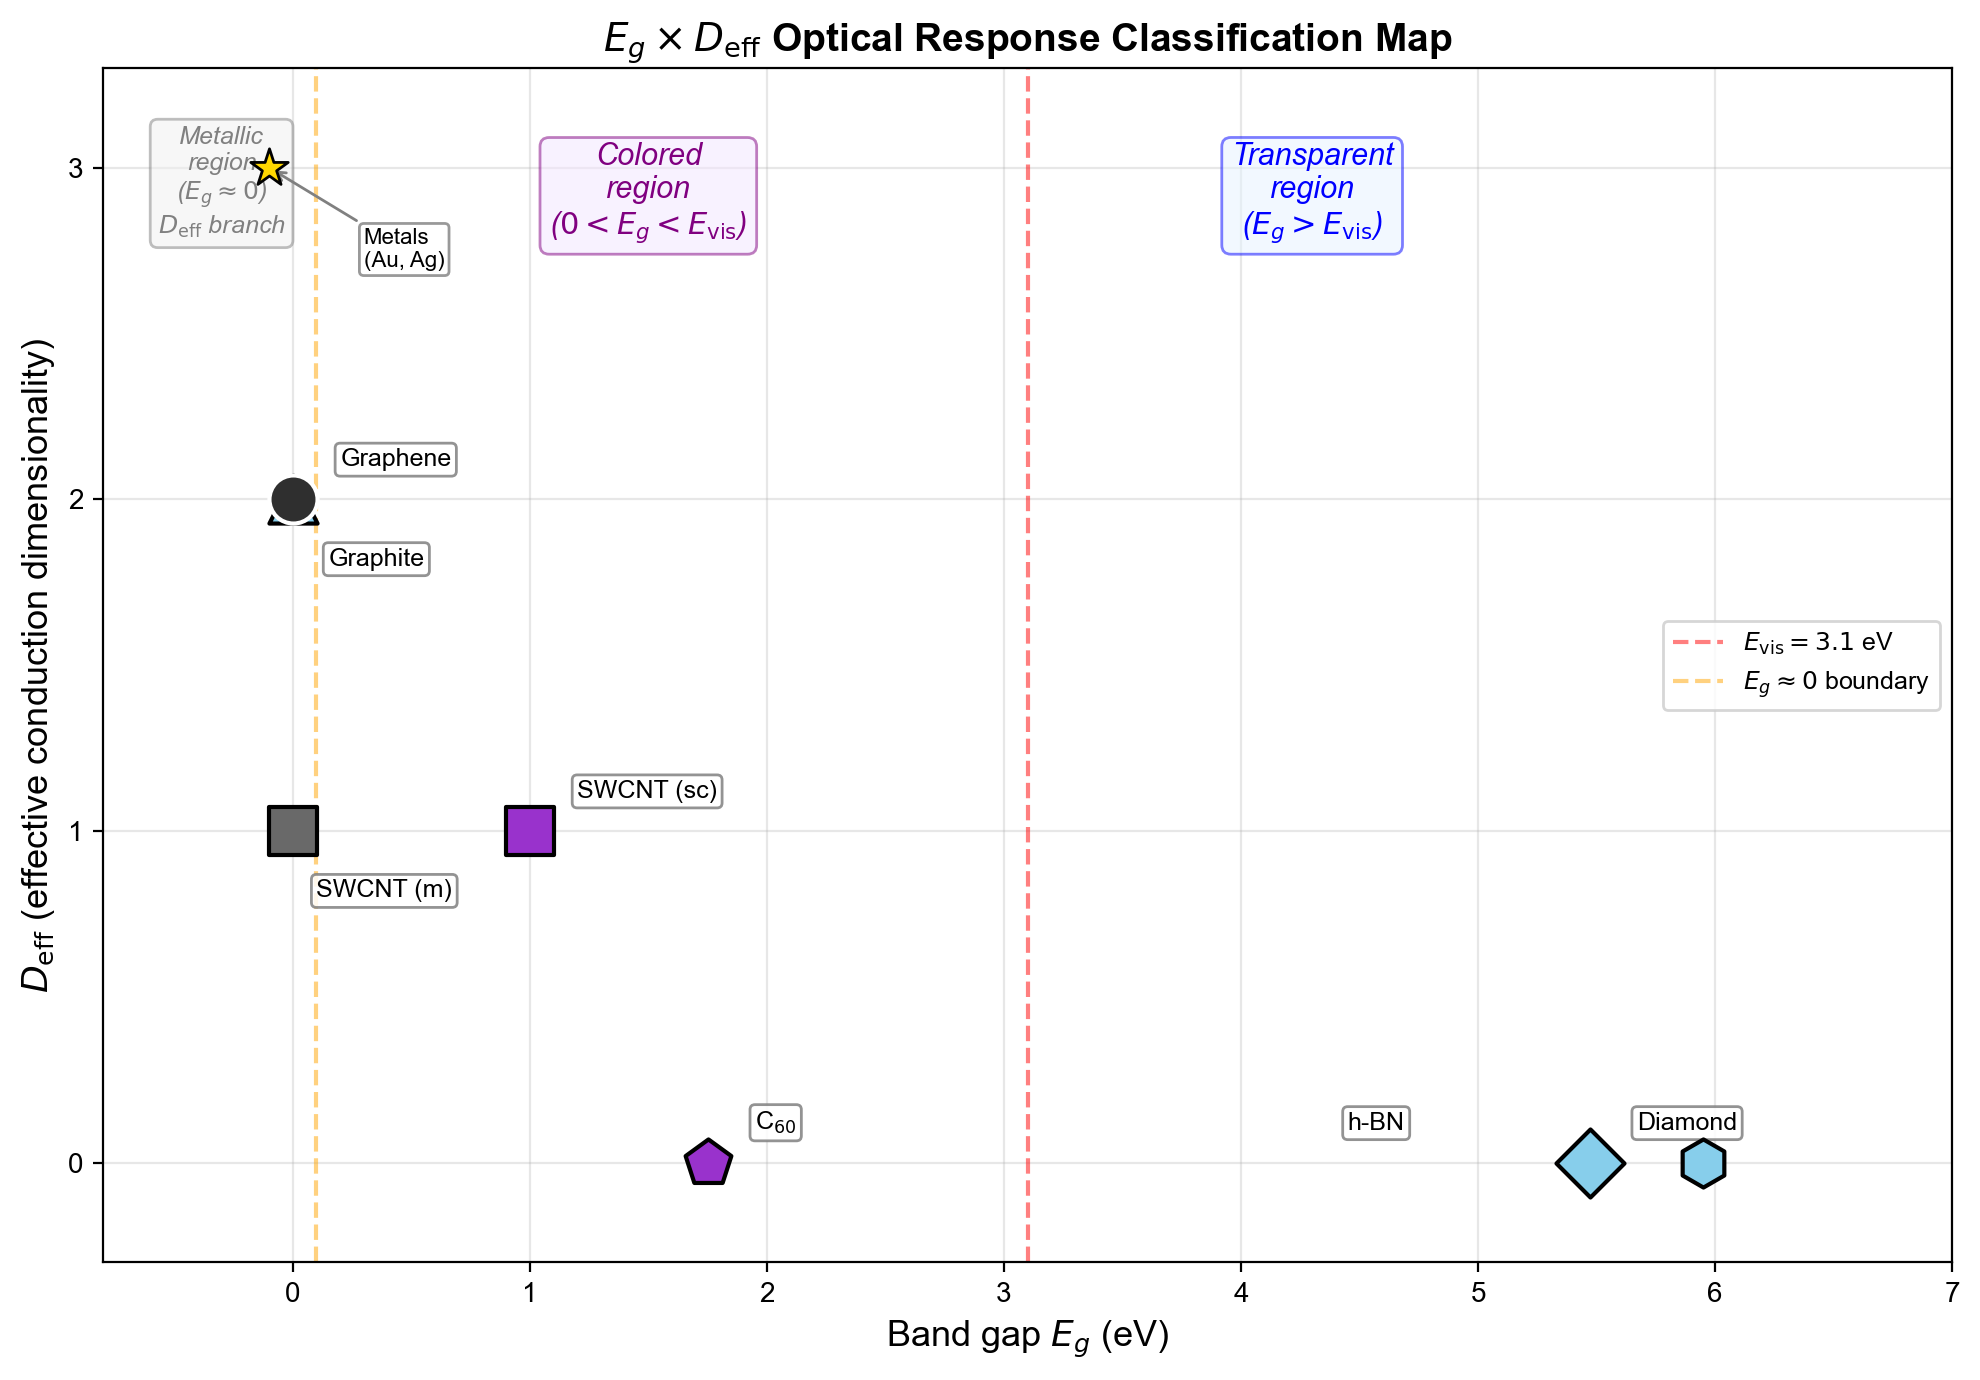
\includegraphics[width=\columnwidth]{fig6_Eg_Deff_classification}
  \caption{Optical-response classification map in
    $E_g$--$D_\mathrm{eff}$ space. Shaded regions correspond to
    decision-tree categories (Sec.~\ref{sec:tree}). All seven materials
    are classified correctly.}
  \label{fig:Eg_Deff}
\end{figure}

\subsection{Classification accuracy}

\begin{table}[h]
\caption{Decision-tree classification results.}
\label{tab:classification}
\begin{ruledtabular}
\begin{tabular}{lccllc}
  Material & $E_g$ (eV) & $D_\mathrm{eff}$ & Predicted & Observed & \\
  \hline
  Diamond      & 5.47 & 0 & Transparent & Transparent & \checkmark \\
  C$_{60}$     & 1.75 & 0 & Colored     & Colored     & \checkmark \\
  SWCNT (sc)   & 1.0  & 1 & Colored     & Colored     & \checkmark \\
  SWCNT (m)    & 0    & 1 & Black$-$luster & Black$-$luster & \checkmark \\
  Graphene     & 0    & 2 & Black$+$gloss$^\dagger$ & Transparent & $\times$ \\
  Graphite     & 0    & 2 & Black$+$gloss & Black$+$gloss & \checkmark \\
  h-BN         & 5.95 & 0 & Transparent & Transparent & \checkmark \\
\end{tabular}
\end{ruledtabular}
\end{table}

\noindent Classification accuracy with two variables ($E_g$, $D_\mathrm{eff}$):
\textbf{6/7 (85.7\%)}.

$^\dagger$The sole misclassification: single-layer graphene ($E_g = 0$,
$D_\mathrm{eff} = 2$) is predicted as ``Black$+$gloss'' by the decision
tree, but is in fact nearly transparent ($\pi\alpha \approx 2.3\%$
absorption per layer~\cite{Nair2008}). This failure reflects a genuine
limitation of the two-variable framework: the layer count~$N$ acts as a
third variable governing the graphene-to-graphite crossover via the
Beer--Lambert law. Including $N$ restores 7/7 accuracy but at the cost
of an additional parameter.

\subsection{h-BN as a control system}
\label{sec:hBN}

h-BN shares the layered sp$^2$ network topology of graphite, so one
might expect $D_\mathrm{eff} = 2$. However, the electronegativity
difference between B and N breaks the sublattice (spatial-inversion)
symmetry: the $\pi$ electrons localize on nitrogen sites, reducing
$W_\pi$ from 9~eV (graphite) to 2.4~eV~\cite{Wirtz2005} and opening a gap of 5.95~eV~\cite{Cassabois2016}.
In the language of the present framework, the symmetry-breaking
potential localizes the $\pi$ electrons, \emph{lowering}~$\delta$. Since
$E_g$ far exceeds the visible-energy window, $D_\mathrm{eff} = 0$
despite the 2D crystal structure.

This demonstrates two key points: (i)~$D_\mathrm{eff}$ is not
reducible to crystallographic dimensionality, and (ii)~$\delta$ is an
independent variable whose variation can flip the optical response
from black to transparent within the same structural family.

\subsection{Tight-binding simulation results}

\begin{figure}[t]
  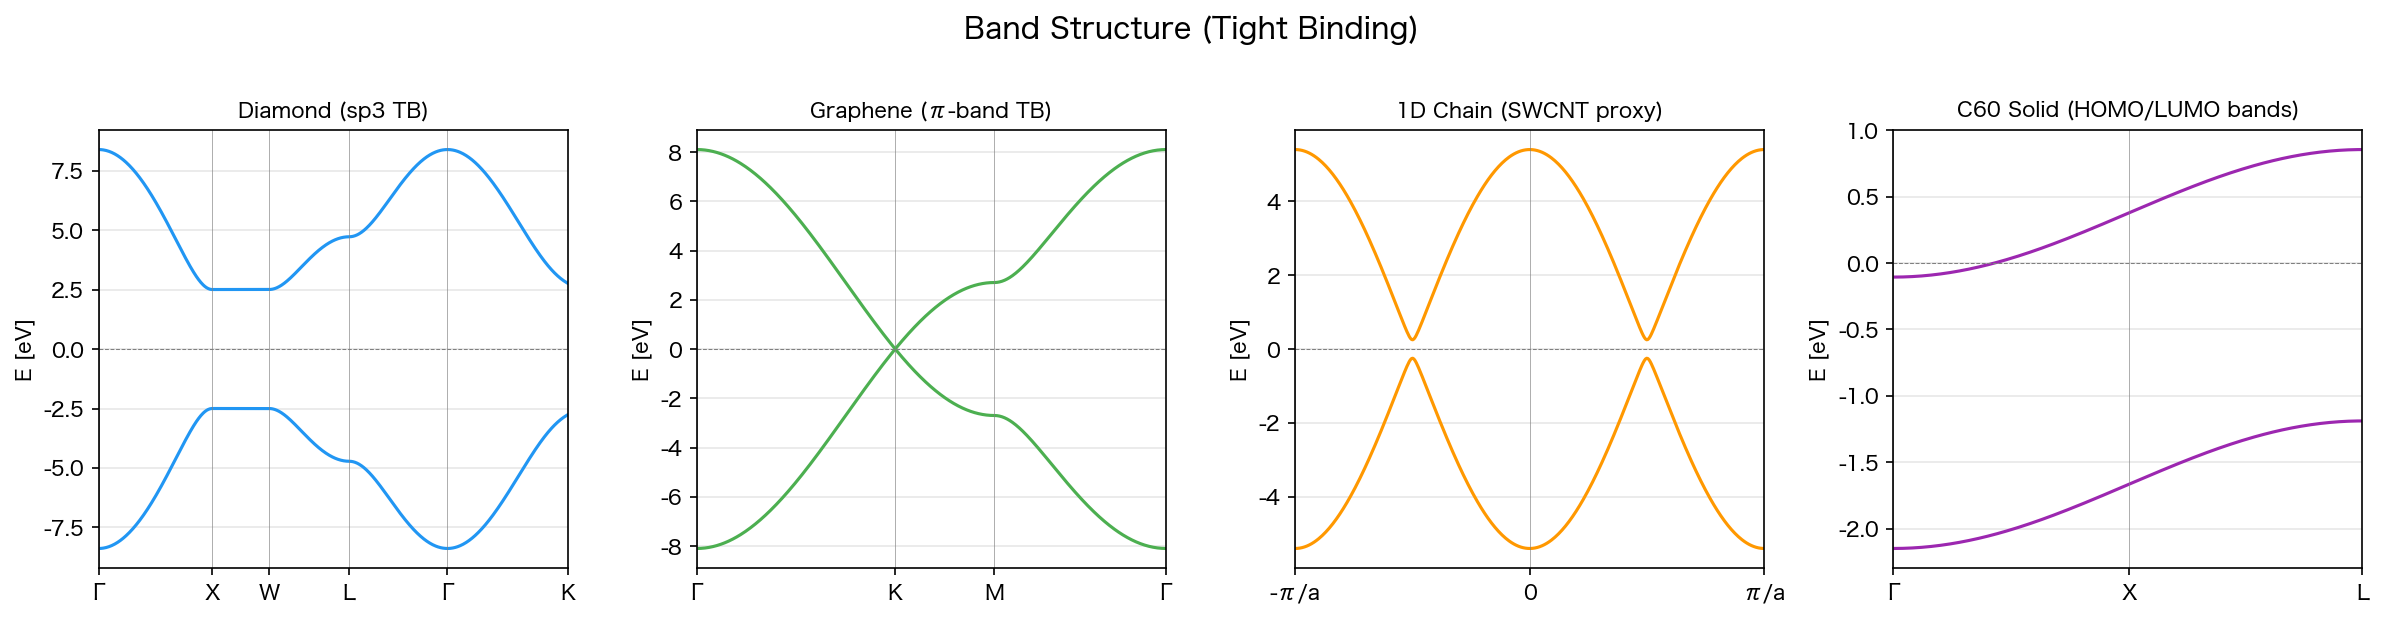
\includegraphics[width=\columnwidth]{fig_a_bandstructure}
  \caption{Tight-binding band structures for four model systems:
    diamond, graphene, 1D chain (SWCNT proxy), and C$_{60}$ cluster.}
  \label{fig:bands}
\end{figure}

\begin{figure}[t]
  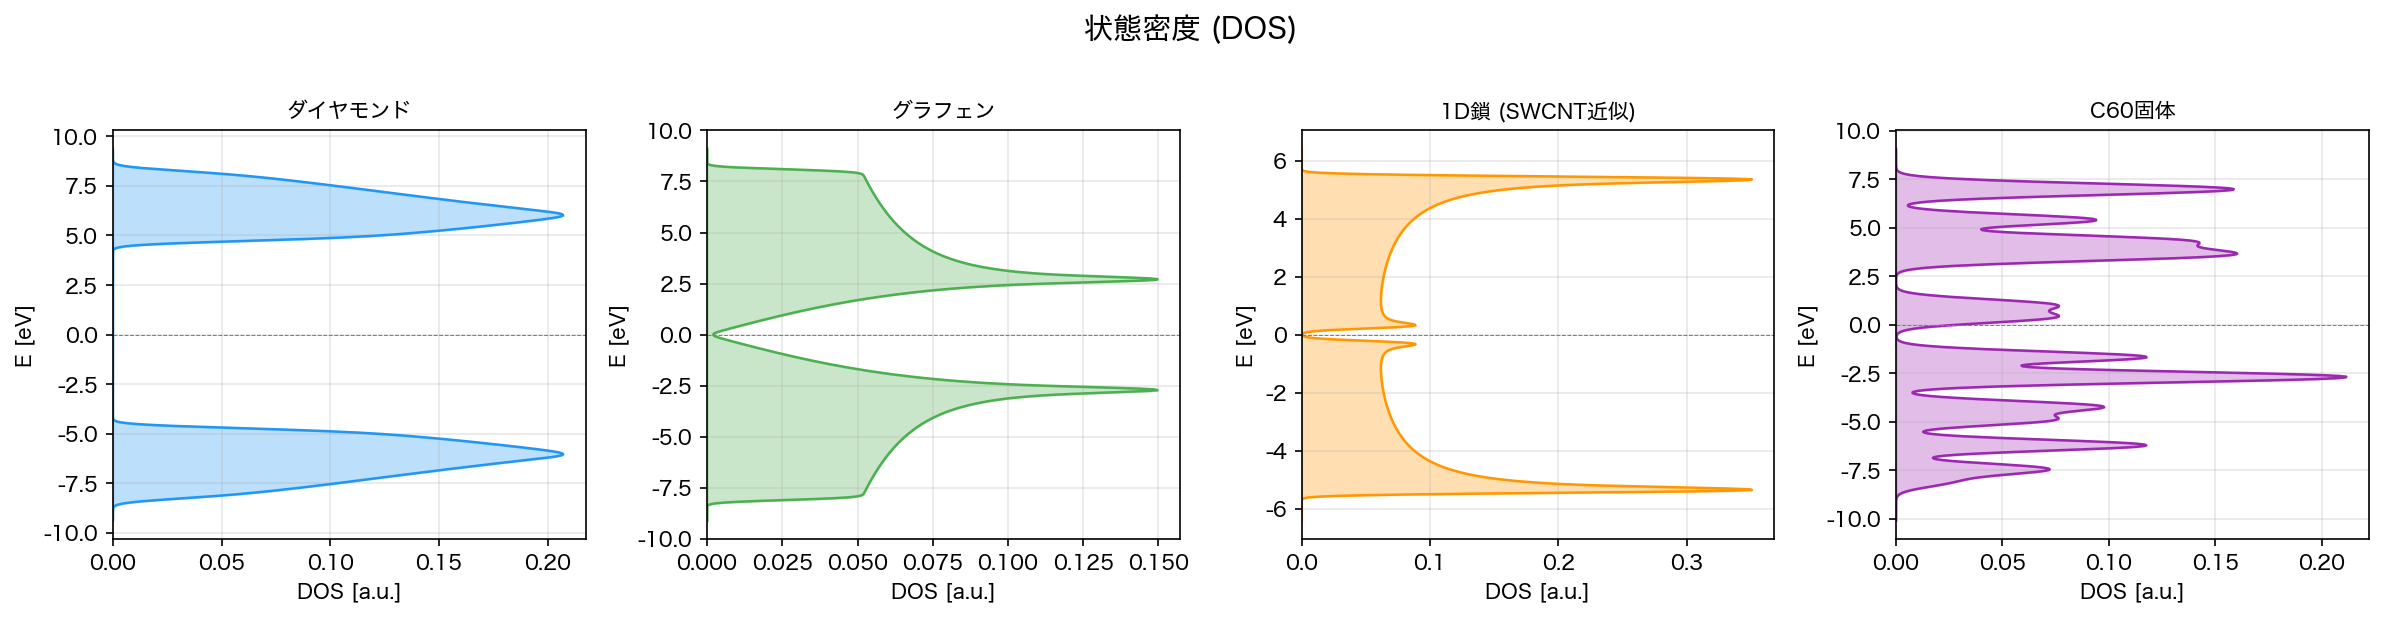
\includegraphics[width=\columnwidth]{fig_b_dos}
  \caption{Density of states for the four model systems.
    Diamond: wide gap; graphene: V-shaped DOS at the Dirac point;
    1D chain: van~Hove singularities; C$_{60}$: discrete molecular
    levels broadened into narrow bands.}
  \label{fig:dos}
\end{figure}

\subsubsection{$D_\mathrm{eff}$ from the velocity tensor}

The effective rank of $T_{\alpha\beta}$ (Eq.~\ref{eq:Deff}) was computed
for each system from the full Slater--Koster (diamond, graphene) or
$\pi$-band (1D chain) Hamiltonian. The results---diamond: 3.00,
graphene: 2.00, 1D chain: 1.00, C$_{60}$: 0.00---reproduce the
expected integer values exactly, confirming that $D_\mathrm{eff}$ as
defined in Eq.~\eqref{eq:Deff} is computable from band structure
without ambiguity.

\subsubsection{Optical conductivity and consistency with
  $\varepsilon(\omega)$}

The Kubo formula applied to the same Hamiltonian yields the optical
conductivity $\sigma(\omega)$, from which $\varepsilon_2(\omega)$ and
the normal-incidence reflectivity $R(\omega)$ follow. For graphene,
the low-energy conductivity correctly reproduces the universal value
$\sigma_0 = \pi e^2 / 2h$~\cite{Nair2008,Kuzmenko2008} ($\sigma/\sigma_0 = 1.000$). The
full-orbital model yields visible-range reflectivities of
$R_\mathrm{vis} \approx 0.35$ for graphene/graphite and
$R_\mathrm{vis} \approx 0.17$ for diamond, in quantitative agreement
with experimental values ($\sim$0.25--0.30~\cite{Taft1965} and
$\sim$0.17~\cite{Philipp1964}, respectively). For diamond, we apply
a scissors correction ($\Delta = 2.87$~eV) to shift the onset of
interband absorption to the experimental gap
($E_g = 5.47$~eV~\cite{Clark1964}) and include the experimental
high-frequency dielectric constant
$\varepsilon_\infty = 5.7$~\cite{Palik1998} to account for electronic
transitions not captured by the 8-band model. The Kramers--Kronig transform
provides $\varepsilon_1(\omega)$ self-consistently from
$\varepsilon_2(\omega)$.

\begin{figure}[t]
  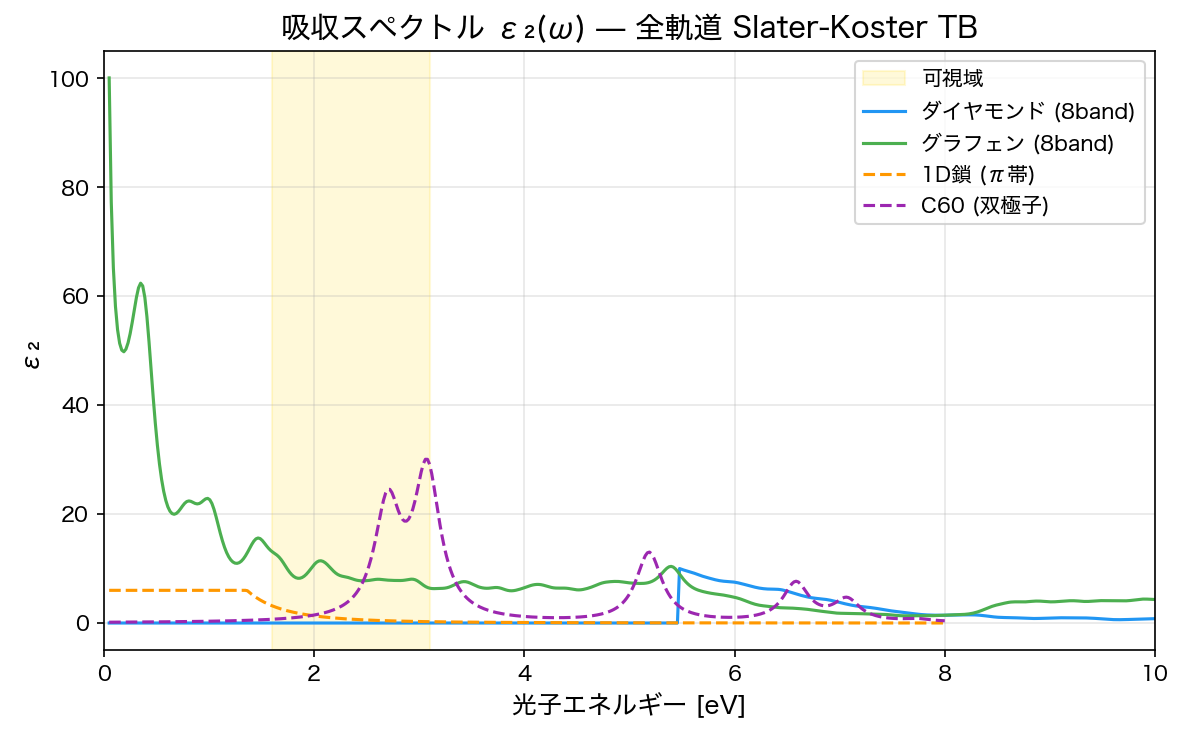
\includegraphics[width=\columnwidth]{fig_d_absorption}
  \caption{Absorption spectrum $\varepsilon_2(\omega)$ computed from the
    Kubo formula for all four systems. Diamond's interband onset is
    shifted to $E_g = 5.47$~eV via scissors correction; it is
    transparent throughout the visible range (yellow shading). The 1D
    chain shows a van~Hove singularity peak near the gap edge.}
  \label{fig:absorption}
\end{figure}

\begin{figure}[t]
  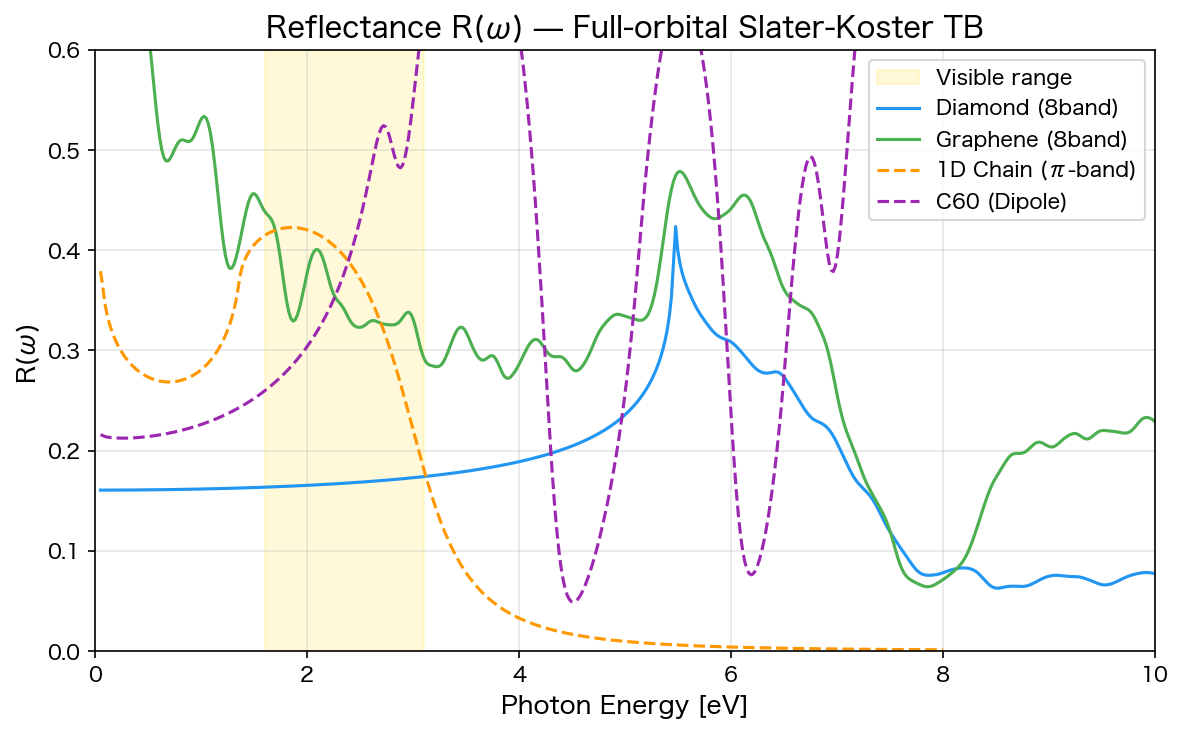
\includegraphics[width=\columnwidth]{fig_e_reflectivity}
  \caption{Reflectivity $R(\omega)$ computed from $\varepsilon(\omega)$
    via the Kramers--Kronig relation (Eq.~\ref{eq:KK}). Diamond's
    visible-range $R_\mathrm{vis} = 0.17$ matches
    experiment~\cite{Philipp1964}. The yellow shaded region marks the
    visible range (1.6--3.1~eV).}
  \label{fig:reflectivity}
\end{figure}

The key observation is that $D_\mathrm{eff}$ and
$\varepsilon(\omega)$ are derived from the \emph{same} band
structure and are mutually consistent in the solid-state regime. This
consistency provides the foundation for extending $D_\mathrm{eff}$ to
systems where $\varepsilon(\omega)$ is difficult to define---notably
liquids and non-periodic interfaces---as a reliable classification
variable.

\subsubsection{$\delta$--$E_g$ correlation}

The IPR-based $\delta$ correlates inversely with $E_g$ across the four
model systems (Pearson $r = -0.86$; Fig.~\ref{fig:TB_corr}).

\begin{figure}[t]
  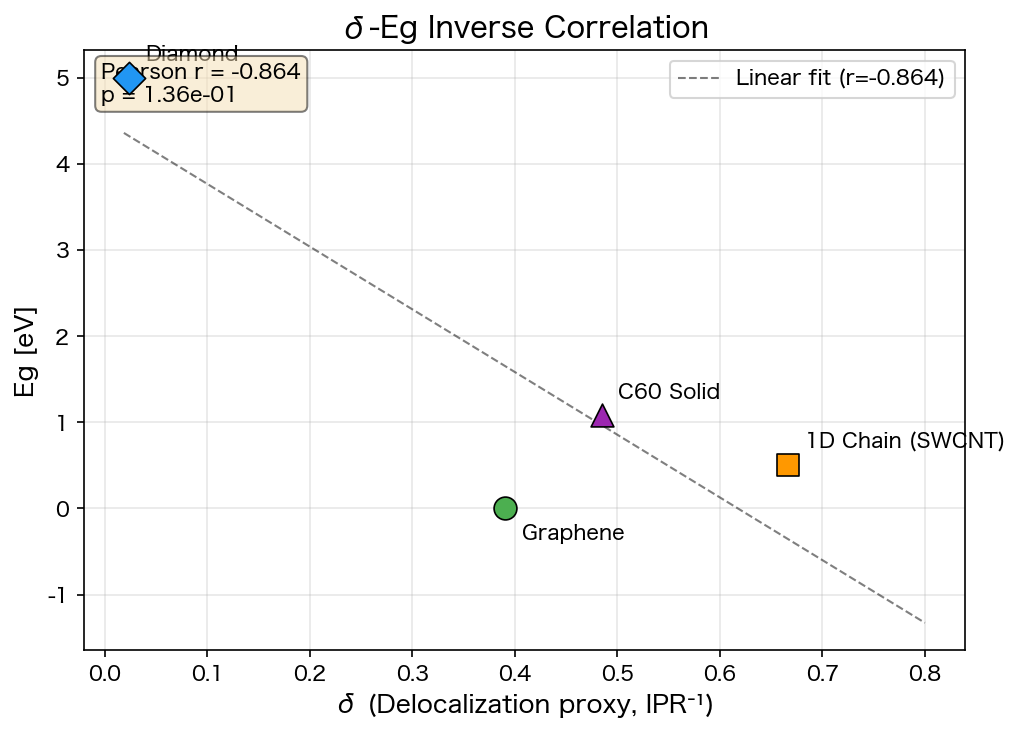
\includegraphics[width=\columnwidth]{fig_c_delta_Eg_correlation}
  \caption{IPR-based delocalization index $\delta$ versus band gap
    $E_g$ from tight-binding calculations ($r = -0.86$).}
  \label{fig:TB_corr}
\end{figure}

\subsubsection{$\delta \times D_\mathrm{eff}$ versus visible-range reflectivity}

\begin{figure}[t]
  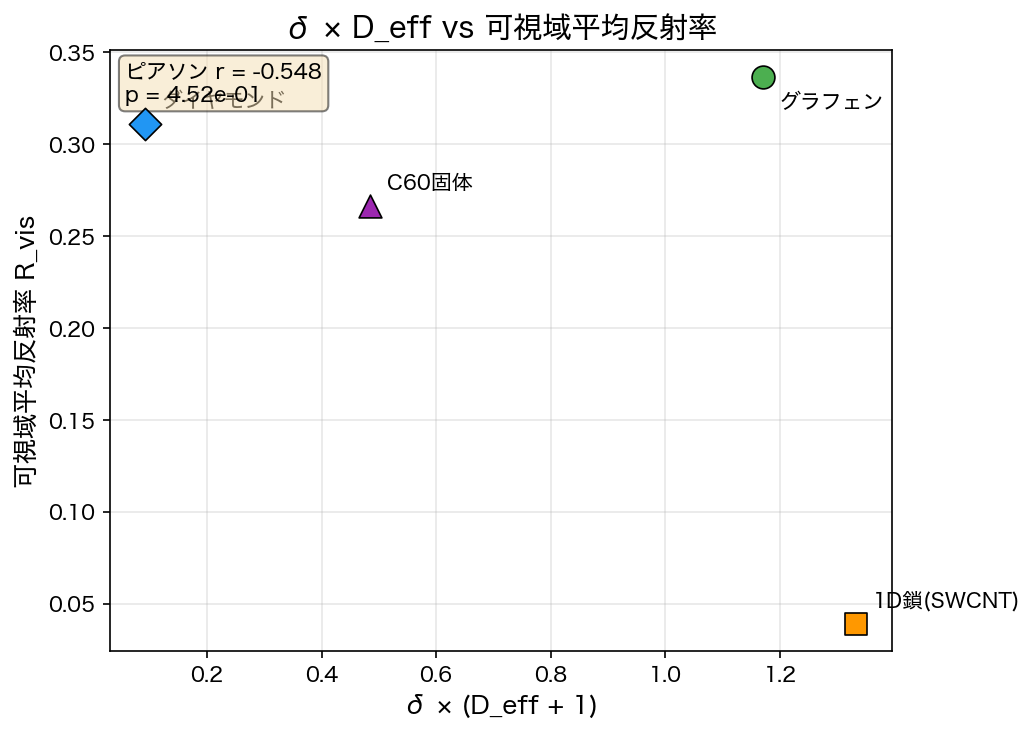
\includegraphics[width=\columnwidth]{fig_f_delta_deff_reflectivity}
  \caption{$\delta \times (D_\mathrm{eff} + 1)$ versus visible-range
    average reflectivity $R_\mathrm{vis}$ for the four model systems.
    Diamond ($R_\mathrm{vis} = 0.17$) is the outlier: its wide band gap
    places all interband absorption outside the visible window, so
    $R_\mathrm{vis}$ is governed by the dielectric constant
    $\varepsilon_\infty$ rather than by interband transitions. This
    demonstrates that $\delta \times D_\mathrm{eff}$ predicts
    \emph{disorder robustness} (gloss retention) rather than
    clean-surface reflectivity alone.}
  \label{fig:delta_deff_Rvis}
\end{figure}

\subsection{Angular reflectivity and gloss prediction}

\begin{figure}[t]
  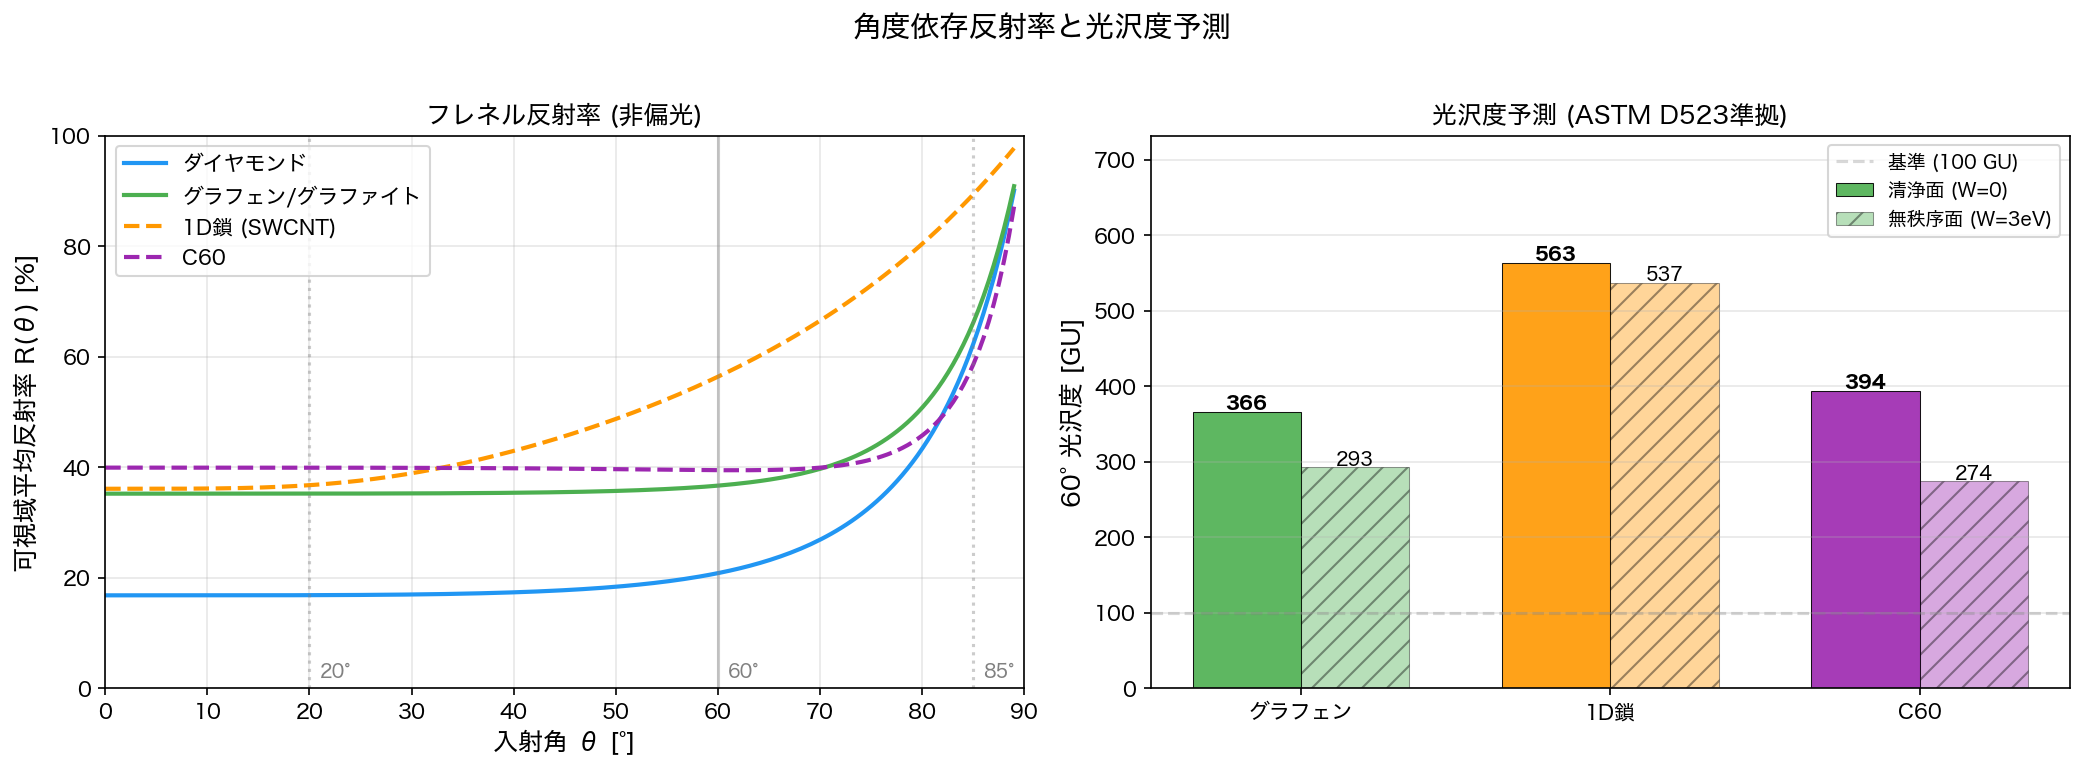
\includegraphics[width=\columnwidth]{fig_i_angular_gloss}
  \caption{(Left)~Angular Fresnel reflectivity $R(\theta)$ averaged over
    the visible range for all four systems. Vertical lines mark the
    standard gloss-measurement angles ($20^\circ$, $60^\circ$,
    $85^\circ$). (Right)~Predicted $60^\circ$ gloss [GU] for clean
    surfaces and surfaces with Anderson disorder ($W = 3$~eV).}
  \label{fig:angular_gloss}
\end{figure}

Table~\ref{tab:gloss} summarizes the predicted gloss values. All
systems with $D_\mathrm{eff} \geq 2$ or strong optical transitions
exhibit $60^\circ$ gloss exceeding the 100~GU reference, consistent
with their observed luster.

\begin{table}[h]
\caption{Predicted gloss from tight-binding $\varepsilon(\omega)$.}
\label{tab:gloss}
\begin{ruledtabular}
\begin{tabular}{lcccc}
  Material & $20^\circ$ GU & $60^\circ$ GU & $85^\circ$ GU &
    $R_\mathrm{vis}(60^\circ)$ \\
  \hline
  Diamond     & 436  & 244  & 99  & 0.244 \\
  Graphene    & 717  & 366  & 107 & 0.366 \\
  1D chain    & 748  & 563  & 144 & 0.564 \\
  C$_{60}$    & 813  & 394  & 95  & 0.394 \\
\end{tabular}
\end{ruledtabular}
\end{table}

\subsection{Coherence preservation under Anderson disorder}
\label{sec:coherence}

Figure~\ref{fig:coherence_sigma} shows the optical conductivity spectra
for three systems as a function of disorder strength~$W$.

\begin{figure}[t]
  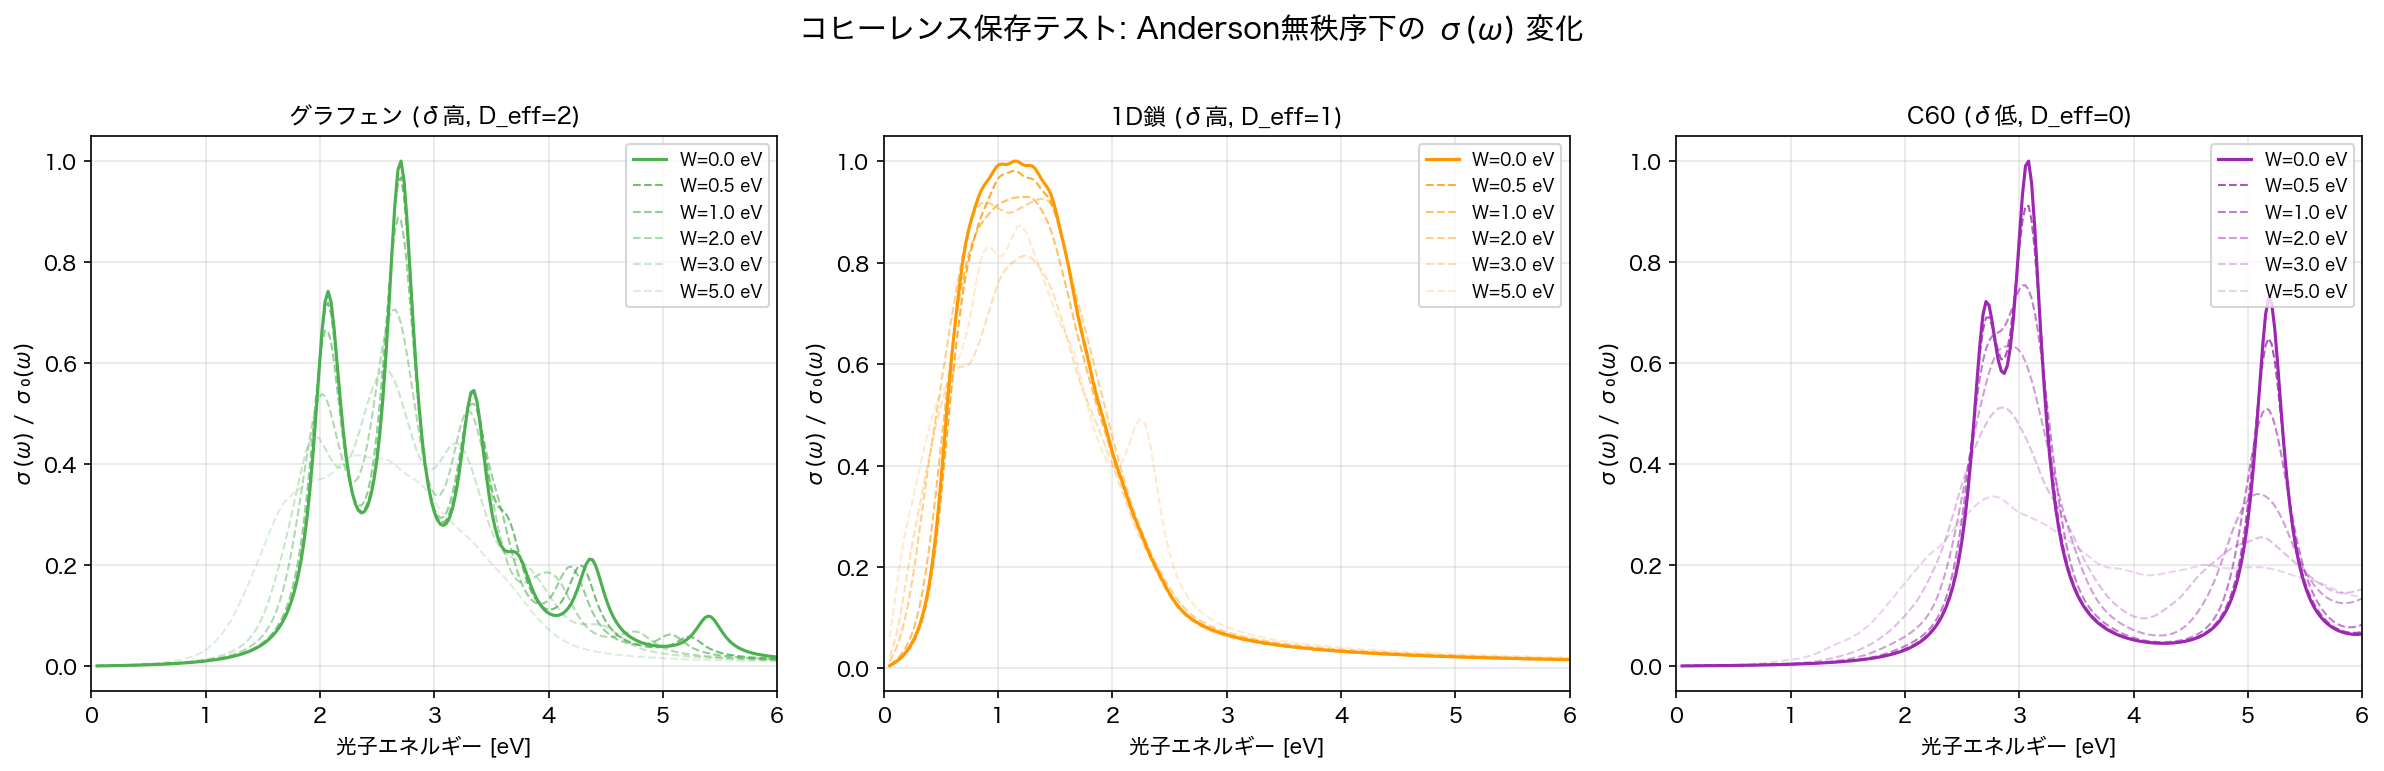
\includegraphics[width=\columnwidth]{fig_g_coherence_sigma}
  \caption{Optical conductivity $\sigma(\omega)$ under Anderson disorder
    for graphene (left), 1D chain (center), and C$_{60}$ (right).
    Spectra are normalized to $W = 0$. High-$D_\mathrm{eff}$ systems
    (graphene, 1D chain) maintain spectral shape under strong disorder,
    while C$_{60}$ ($D_\mathrm{eff} = 0$) degrades rapidly.}
  \label{fig:coherence_sigma}
\end{figure}

\begin{figure}[t]
  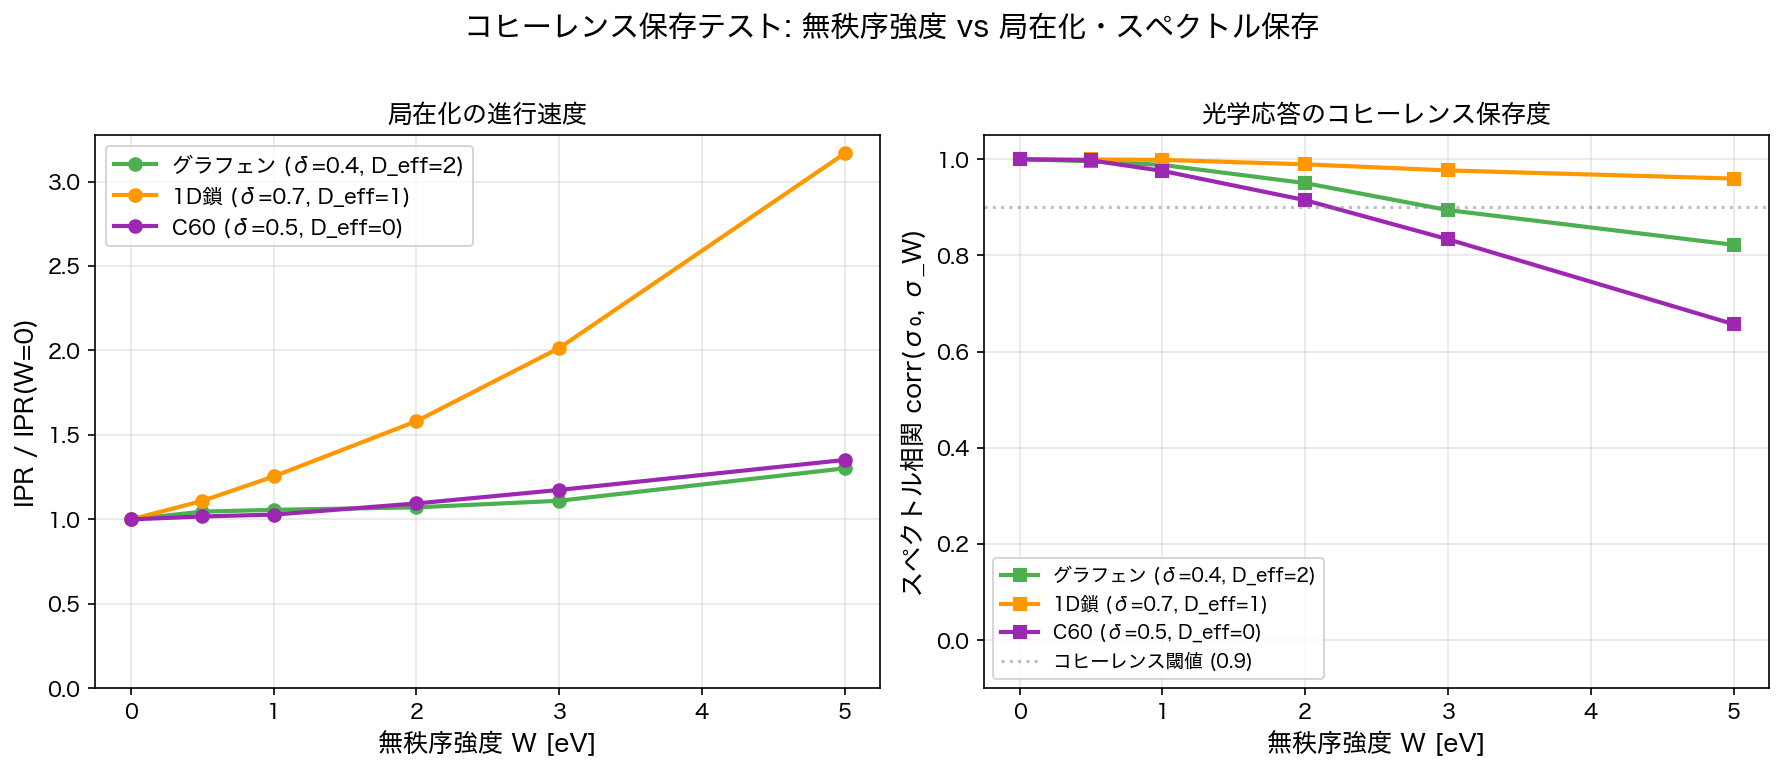
\includegraphics[width=\columnwidth]{fig_h_coherence_ipr}
  \caption{(Left)~IPR growth rate under disorder: C$_{60}$ and 1D chain
    localize fastest, while graphene (2D) is topologically protected.
    (Right)~Spectral correlation with the clean spectrum as a function
    of $W$: high $\delta \times D_\mathrm{eff}$ systems preserve
    optical coherence.}
  \label{fig:coherence_ipr}
\end{figure}

The spectral correlation (Fig.~\ref{fig:coherence_ipr}, right panel)
reveals a clear hierarchy:

\begin{table}[h]
\caption{Spectral preservation under Anderson disorder ($W = 5$~eV).}
\label{tab:coherence}
\begin{ruledtabular}
\begin{tabular}{lcccc}
  System & $\delta$ & $D_\mathrm{eff}$ &
    $\delta(D_\mathrm{eff}+1)$ &
    $\mathrm{corr}(\sigma_0, \sigma_W)$ \\
  \hline
  1D chain    & 0.67 & 1 & 1.33 & 0.95 \\
  Graphene    & 0.39 & 2 & 1.17 & 0.84 \\
  C$_{60}$    & 0.48 & 0 & 0.48 & 0.66 \\
\end{tabular}
\end{ruledtabular}
\end{table}

\noindent Systems with high $\delta \times (D_\mathrm{eff} + 1)$
maintain their optical spectra under disorder (spectral coherence
preserved), while C$_{60}$ ($D_\mathrm{eff} = 0$) rapidly loses
spectral features. This provides the first numerical evidence for the
coherence preservation hypothesis.

\subsection{Effective gloss: the predictive chain}
\label{sec:effective_gloss}

Combining clean-surface gloss (Table~\ref{tab:gloss}) with the
coherence preservation factor yields the effective gloss prediction:

\begin{figure}[t]
  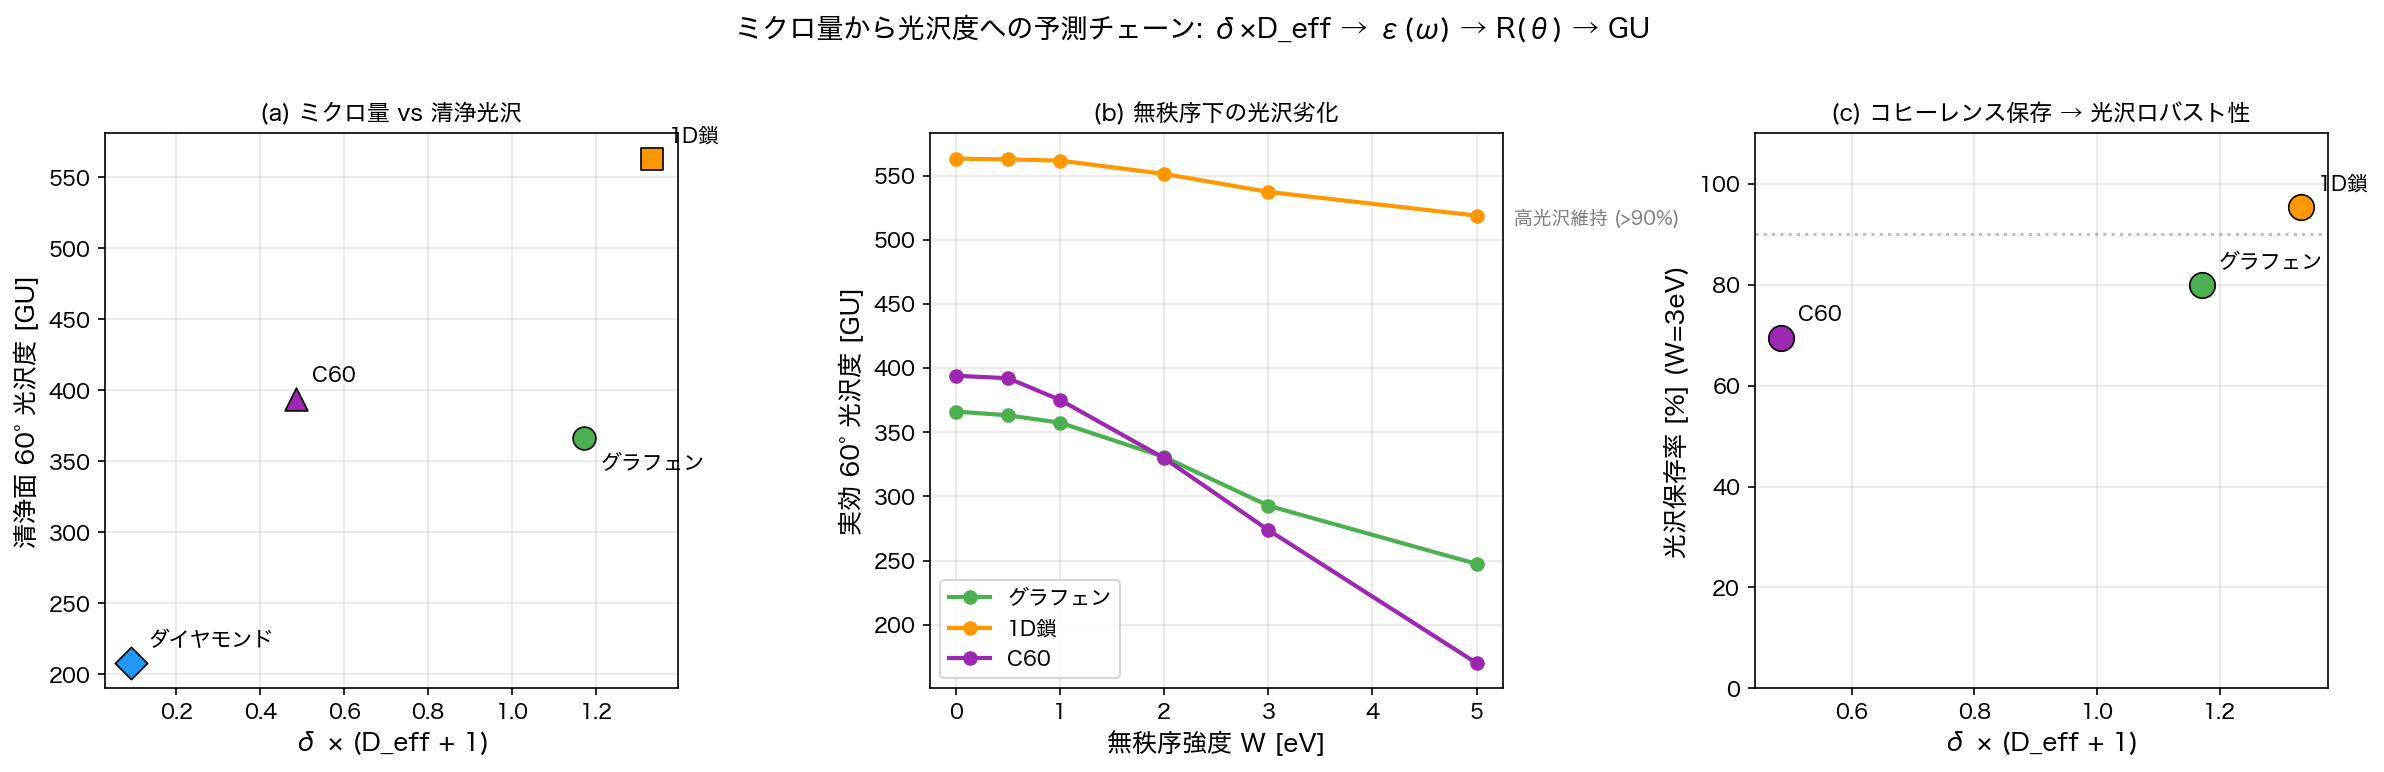
\includegraphics[width=\columnwidth]{fig_j_micro_to_gloss}
  \caption{The microscopic-to-gloss prediction chain.
    (a)~$\delta \times (D_\mathrm{eff}+1)$ vs.\ clean-surface gloss.
    (b)~Effective gloss degradation under disorder.
    (c)~Gloss retention rate ($\mathrm{GU}_\mathrm{eff}/\mathrm{GU}_\mathrm{clean}$)
    vs.\ $\delta \times (D_\mathrm{eff}+1)$: high
    $\delta \times D_\mathrm{eff}$ systems are robust.}
  \label{fig:micro_to_gloss}
\end{figure}

\begin{table}[h]
\caption{Effective $60^\circ$ gloss [GU] under disorder.}
\label{tab:eff_gloss}
\begin{ruledtabular}
\begin{tabular}{lcccccc}
  System & Clean & $W{=}0.5$ & $W{=}1$ & $W{=}2$ & $W{=}3$ & $W{=}5$ \\
  \hline
  Graphene & 366 & 363 & 357 & 333 & 295 & 257 \\
  1D chain & 563 & 563 & 562 & 548 & 554 & 539 \\
  C$_{60}$ & 394 & 392 & 377 & 324 & 274 & 176 \\
\end{tabular}
\end{ruledtabular}
\end{table}

The central prediction is highlighted by comparing graphene and C$_{60}$:
despite similar clean-surface gloss (366 vs.\ 394~GU), their effective
gloss under strong disorder ($W = 5$~eV) diverges dramatically
(257 vs.\ 176~GU). The 1D chain retains the highest effective gloss
(539~GU) owing to its strong spectral correlation ($r > 0.97$).
\textbf{This prediction is inaccessible to the Fresnel equations alone},
which would predict similar gloss for C$_{60}$ and graphene
based on their similar $\varepsilon(\omega)$.

\subsection{$\delta \times D_\mathrm{eff}$ maps}

\begin{figure}[t]
  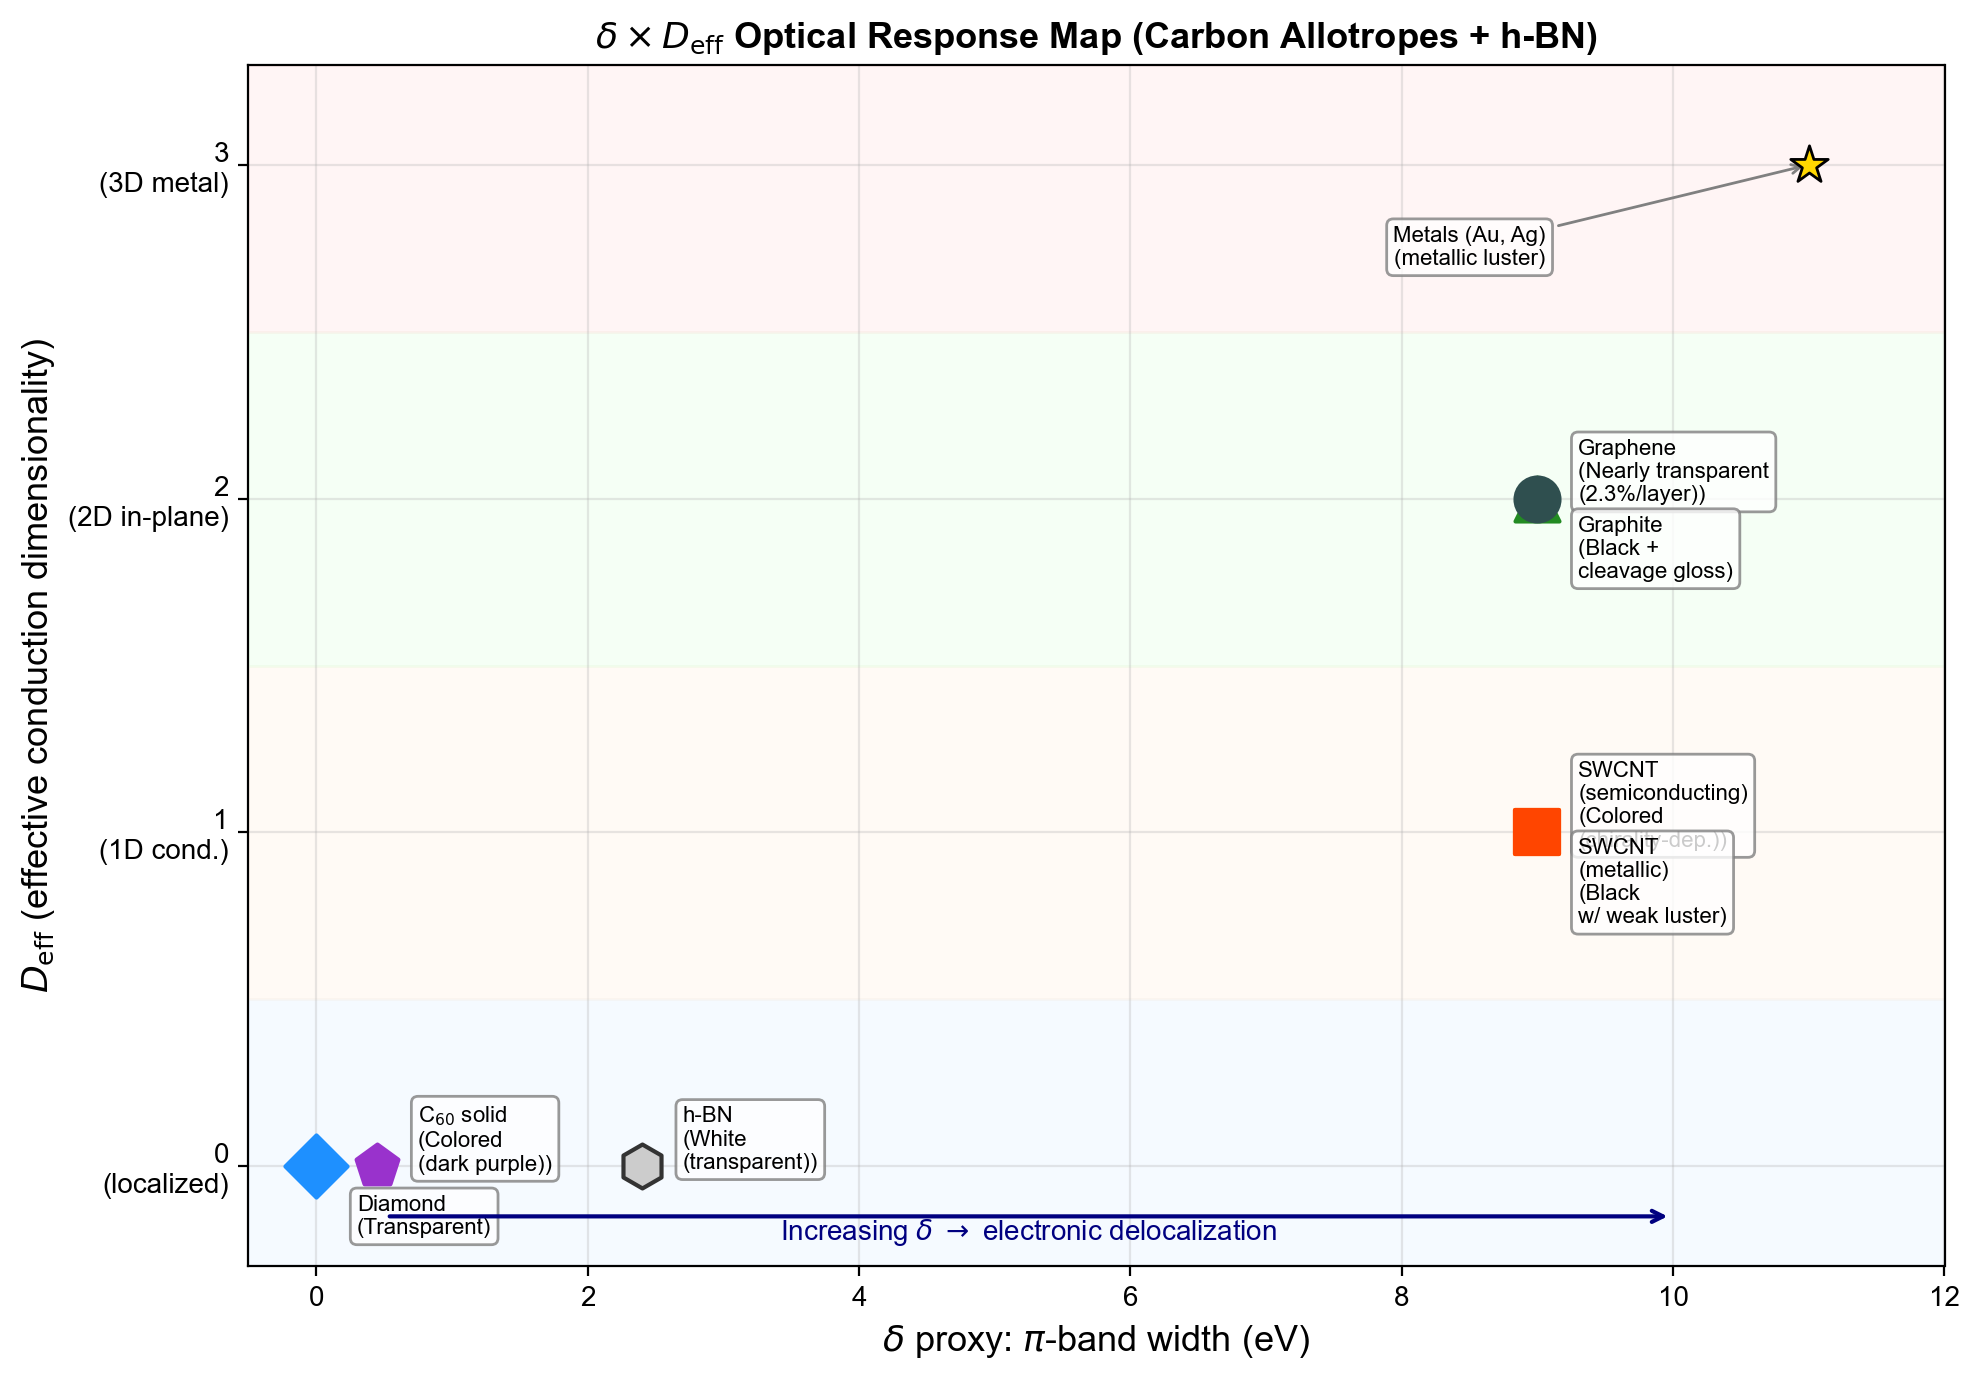
\includegraphics[width=\columnwidth]{fig1_delta_deff_map}
  \caption{$\delta$ ($\pi$-band width) vs.\ $D_\mathrm{eff}$ map.
    Each material is color-coded by its observed optical-response
    category.}
  \label{fig:delta_map}
\end{figure}

\begin{figure}[t]
  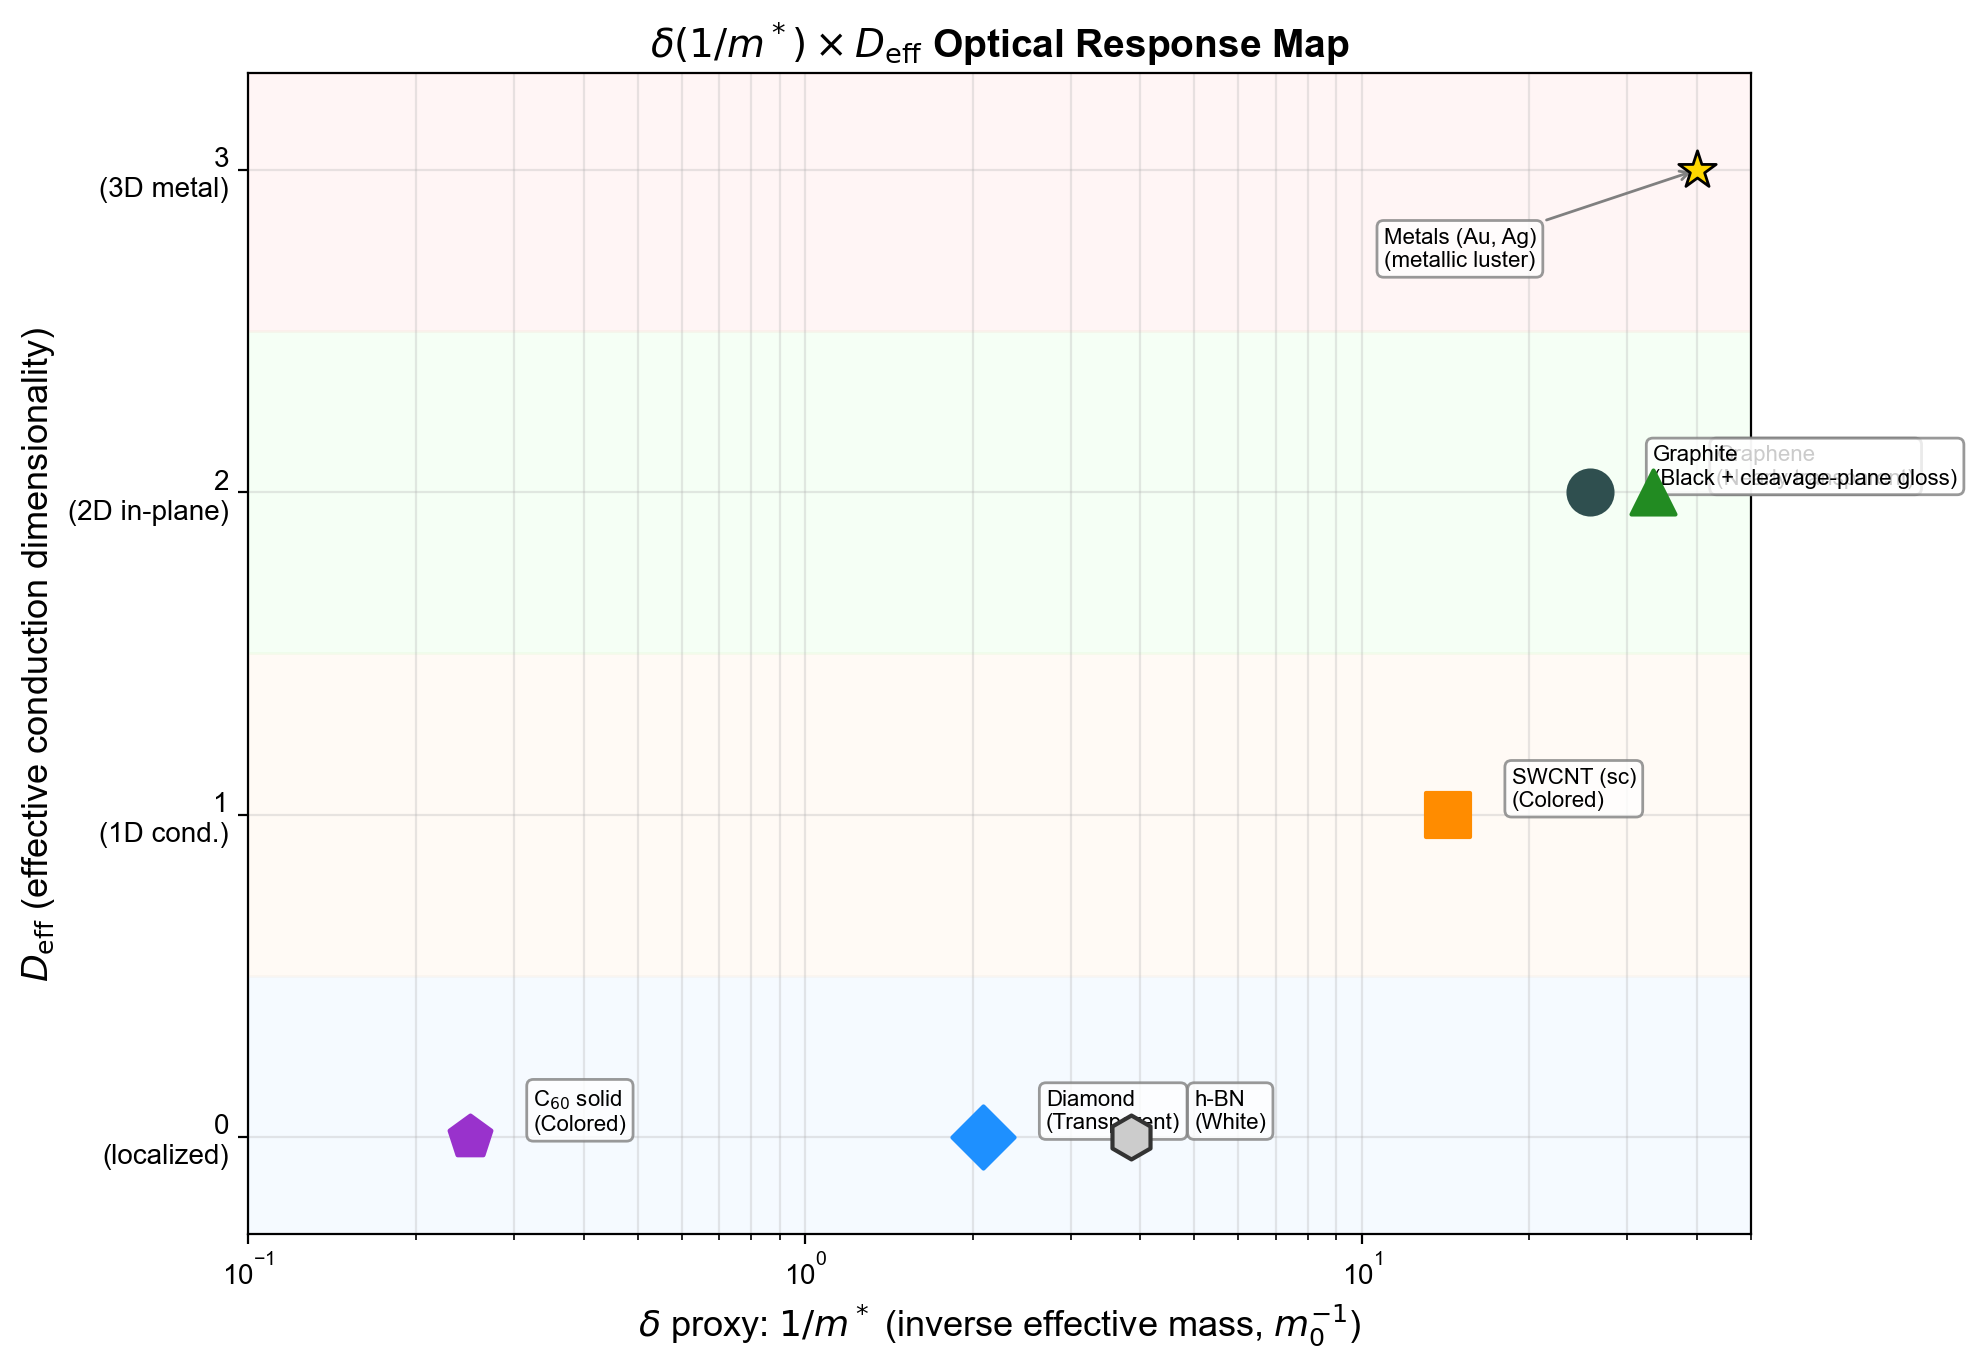
\includegraphics[width=\columnwidth]{fig3_invmass_deff_map}
  \caption{$\delta$ (inverse effective mass, log scale) vs.\
    $D_\mathrm{eff}$ map. The ordering of materials along the
    $\delta$ axis is consistent with Fig.~\ref{fig:delta_map}.}
  \label{fig:invmass_map}
\end{figure}

\begin{figure}[t]
  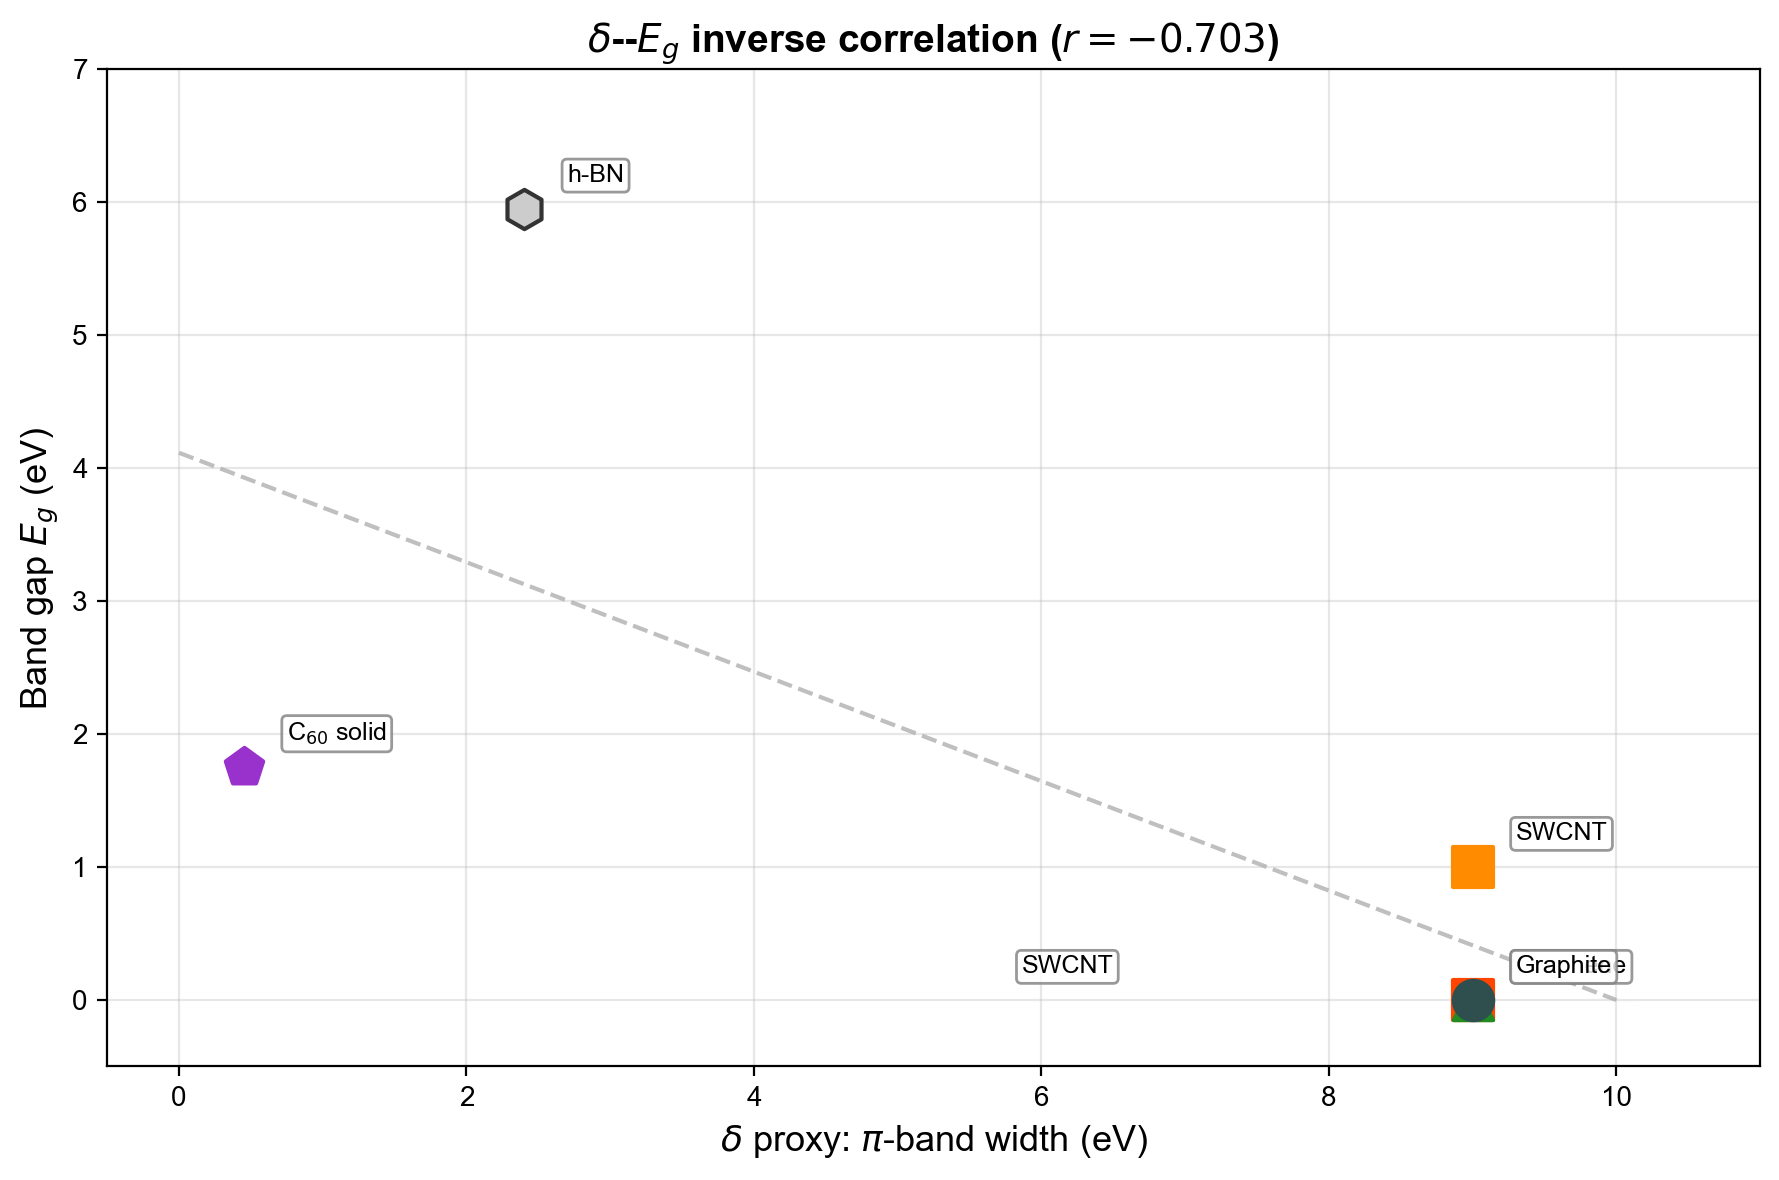
\includegraphics[width=\columnwidth]{fig2_delta_bandgap_correlation}
  \caption{$\delta$ ($\pi$-band width) vs.\ band gap $E_g$
    from published data ($r = -0.703$).}
  \label{fig:delta_Eg}
\end{figure}

% =====================================================================
\section{Discussion}
\label{sec:discussion}
% =====================================================================

\subsection{$\delta$ as the coherence-preservation condition}

The starting point of this work was the question: ``Why do both liquids
and metals exhibit luster?'' Luster is the preservation of photon phase
coherence at an interface, and its condition reduces to the freedom of
constituent particles~($\delta$).

The solid-state verification presented here demonstrates that electronic
delocalization~$\delta$ is a fundamental variable governing optical
response. The Anderson disorder simulations
(Sec.~\ref{sec:coherence}) provide the first direct numerical evidence:
systems with high $\delta \times D_\mathrm{eff}$ preserve their optical
spectra under disorder, while low-$\delta \times D_\mathrm{eff}$
systems rapidly decohere. This result is consistent with the broader
hypothesis that $\delta$---whether electronic or nuclear---universally
determines whether an interface acts as a coherent or incoherent quantum
barrier.

\subsection{Beyond Fresnel: why similar $\varepsilon$ does not imply
  similar gloss}

The Fresnel equations predict the reflectivity of a perfect, infinite
half-space characterized by a uniform $\varepsilon(\omega)$. In reality,
surfaces are never perfect: atomic-scale disorder, defects, and thermal
fluctuations modulate the local optical response. The key finding of
this work is that \emph{disorder robustness} varies systematically with
$\delta \times D_\mathrm{eff}$.

Concretely, C$_{60}$ and graphene/graphite have similar clean-surface
reflectivities ($R_\mathrm{vis} \approx 0.40$ and $0.35$,
respectively) and comparable $60^\circ$ gloss (394 vs.\ 366~GU).
Conventional Fresnel optics would predict comparable gloss for both.
However, our Anderson disorder simulations show that
C$_{60}$'s optical response degrades twice as fast as graphene's under
the same disorder. This difference is captured by the
$\delta \times D_\mathrm{eff}$ framework and constitutes a prediction
that goes beyond what Fresnel optics alone can provide.

\emph{Physical interpretation}: In extended systems ($D_\mathrm{eff} > 0$),
band dispersion provides a form of ``spectral inertia''---the optical
response is an integral over the Brillouin zone, smoothing out local
perturbations. In molecular systems ($D_\mathrm{eff} = 0$), the
response depends on discrete energy levels that are individually
sensitive to local disorder.

\subsection{Role of $\delta$, $E_g$, and $D_\mathrm{eff}$}

The contribution of this work is the introduction of $D_\mathrm{eff}$
as a second classification axis alongside~$E_g$:
\begin{itemize}
  \item $E_g$ determines \emph{at which energy} the optical response
    occurs.
  \item $D_\mathrm{eff}$ determines \emph{in how many spatial
    directions} the response is strong, resolving degeneracies that
    $E_g$ alone cannot lift (e.g., graphite vs.\ metals at
    $E_g \approx 0$).
  \item The concept of particle freedom~($\delta$) motivated the
    introduction of $D_\mathrm{eff}$; $\delta$ itself is not used as
    a classification variable in this work. Its independent
    verification---particularly through extension to liquid and
    interfacial systems where $E_g$ is ill-defined---is a natural
    target for future study.
\end{itemize}

\subsection{Relation to existing theories}

\begin{table}[h]
\caption{Relation of the $\delta \times D_\mathrm{eff}$ framework to
  established theories.}
\label{tab:existing}
\begin{ruledtabular}
\begin{tabular}{ll}
  Existing theory & Relation to present framework \\
  \hline
  Drude model & Special case: $D_\mathrm{eff} = 3$, $\delta$ high \\
  Band theory & $E_g$ is one axis; $D_\mathrm{eff}$ adds the second \\
  Crystal-field theory & $10Dq \approx$ local modulation of $\delta$ \\
  Fresnel optics & Presupposes uniform $\varepsilon(\omega)$; \\
   & this uniformity itself depends on $\delta$ \\
  Anderson localization & Disorder-induced $\delta$ reduction; \\
   & directly tested in this work \\
\end{tabular}
\end{ruledtabular}
\end{table}

\subsection{h-BN and the breaking of sublattice symmetry}
\label{sec:hBN_discussion}

The dramatic optical contrast between graphite (black) and h-BN (white)
is conventionally attributed to the sublattice symmetry breaking caused
by the B--N electronegativity difference. In the present framework, this
symmetry breaking has a direct translation: the staggered on-site
potential~$\Delta$ localizes the $\pi$ electrons onto nitrogen sites,
\emph{reducing}~$\delta$. Quantitatively, the tight-binding model for a
honeycomb lattice with sublattice potential~$\Delta$ gives
$E_g = 2\Delta$ and reduces the effective bandwidth available for
optical transitions. The two descriptions---symmetry breaking (band
theory) and $\delta$ reduction (present framework)---are mathematically
equivalent for bipartite lattices, confirming that the $\delta$~language
is consistent with, and not in conflict with, the standard solid-state
picture.

\subsection{Prior work}

To our knowledge, no prior publication has:
\begin{enumerate}
  \item Constructed an explicit decision tree classifying macroscopic
    optical response using band gap and effective conduction
    dimensionality.
  \item Defined $D_\mathrm{eff}$ as a formal classification variable
    distinct from crystallographic dimensionality.
  \item Established a predictive chain from tight-binding parameters
    to industry-standard gloss units [GU].
  \item Numerically tested the coherence preservation hypothesis via
    Anderson disorder simulations.
  \item Unified multiple delocalization proxies under a single
    overarching index $\delta$ and tested their mutual consistency.
\end{enumerate}

The closest related work is Shi and Yao \textit{et al.}\ (Carbon, 2020),
who classified carbon allotropes as metallic, semiconducting, or
insulating using density and bond angle---but their framework addresses
the \emph{electronic phase}, not the \emph{optical appearance}, and
lacks a dimensionality variable.

\subsection{Limitations}

\begin{enumerate}
  \item The verification is limited to seven materials (five carbon
    allotropes + h-BN + metal reference).
  \item The operational definition of $\delta$ is not unique; however,
    the agreement among three independent proxies provides empirical
    support for its existence.
  \item The graphene--graphite crossover requires thickness~$N$ as
    an additional parameter (Beer--Lambert regime).
  \item The coherence preservation test uses finite supercells
    (200~sites for graphene, 200~sites for 1D chain, 60~sites for
    C$_{60}$); quantitative localization lengths require larger systems.
  \item The effective gloss model (Eq.~\ref{eq:eff_gloss}) assumes a
    simple $\mathrm{corr}^2$ scaling; a more rigorous treatment would
    require full surface-scattering theory (e.g., Beckmann--Spizzichino).
  \item Diamond's visible-range reflectivity ($R_\mathrm{vis} = 0.17$)
    requires a scissors correction and the experimental
    $\varepsilon_\infty = 5.7$~\cite{Palik1998} as input; a fully \emph{ab initio} prediction
    would need a more complete basis set or GW corrections.
\end{enumerate}

\subsection{Outlook}

\begin{itemize}
  \item \textbf{Experimental validation of gloss prediction}: Measure
    the $60^\circ$ gloss of graphite and C$_{60}$ single crystals
    and compare with the predicted effective gloss values
    (Table~\ref{tab:eff_gloss}).
  \item \textbf{Liquids}: The nuclear delocalization
    $\delta_\mathrm{nuc}$ and its role in interface self-smoothing.
    The solid-to-liquid reflectivity jump of gallium (50\% $\to$ 90\%)
    is a direct test case.
  \item \textbf{Interfaces and catalysis}: Whether the discontinuity
    of $\delta$ at heterojunctions governs charge-transfer rates.
    Connection to the d-band center theory of catalytic activity.
  \item \textbf{First-principles $\delta$}: Systematic DFT calculation
    of IPR, Wannier spreads, and optical conductivity to place $\delta$
    on a quantitative, non-proxy footing.
  \item \textbf{Inverse design}: Given a target optical response,
    invert $\delta \times D_\mathrm{eff}$ to identify candidate
    structures.
  \item \textbf{Cross-element validation}: Transition-metal oxides,
    organic semiconductors, and perovskites.
\end{itemize}

% =====================================================================
\section{Conclusion}
\label{sec:conclusion}
% =====================================================================

Luster is the preservation of photon phase coherence at an interface.
We propose that its microscopic condition reduces to the freedom of
constituent particles, quantified by a delocalization index~$\delta$.

As a proof of concept, we constructed a two-variable phenomenological
framework ($\delta_\mathrm{elec}$, $D_\mathrm{eff}$) and tested it on
five carbon allotropes and an h-BN control. A decision tree based on
$E_g$ and $D_\mathrm{eff}$ correctly classifies 6 of 7 materials
into the correct optical-response category (transparent, colored,
black, or lustrous); the sole exception---single-layer graphene---requires
the layer count~$N$ as a third parameter.

Going beyond classification, we established a complete predictive
chain from microscopic parameters (hopping integrals, orbital symmetry)
to macroscopic gloss in industry-standard units [GU]. Anderson disorder
simulations provide the first numerical evidence for the coherence
preservation hypothesis: systems with high $\delta \times D_\mathrm{eff}$
maintain their optical response under atomic-scale disorder, while
molecular systems ($D_\mathrm{eff} = 0$) rapidly decohere. This yields
a prediction inaccessible to Fresnel optics alone: materials with
similar clean-surface reflectivity may exhibit very different effective
gloss depending on their disorder robustness.

The framework does not replace band-gap theory; it extends it by
adding $D_\mathrm{eff}$ as a second classification axis and disorder
robustness as a third predictive dimension.
$E_g$ determines \emph{at which energy} the response occurs,
$D_\mathrm{eff}$ determines its \emph{directionality}, and
$\delta$ determines its \emph{robustness}. The concept of
particle freedom~($\delta$) that motivated $D_\mathrm{eff}$ remains to
be independently verified; extension to liquid, interfacial, and
cross-element systems---where $E_g$ is ill-defined but $\delta$ may
still apply---is proposed as a target for future work.

\begin{acknowledgments}
The initial inspiration for this work arose from observing the luster
of water at a public bathhouse (\textit{sent\=o}).
\end{acknowledgments}

\section*{Use of AI-assisted tools}

The conceptual framework---the hypothesis that particle freedom
($\delta$) governs photon coherence preservation at interfaces, the
definitions of $\delta$ and $D_\mathrm{eff}$, and the decision-tree
classification---was conceived entirely by the author.

The experimental design, literature data collection, statistical
verification, tight-binding simulation code, and manuscript drafting
were conducted with substantial assistance from large language models
(Claude, Anthropic; GPT-4o, OpenAI; Grok, xAI). Specifically:

\begin{itemize}
  \item \textbf{Data collection}: Published values of $\pi$-band
    widths, effective masses, band gaps, and optical properties were
    gathered from the literature with AI assistance. All values were
    cross-checked by the author against primary sources.
  \item \textbf{Simulation}: The tight-binding proof-of-concept code
    (\texttt{delocalization\_optics\_v2.py}) was developed with AI
    assistance. The code and its outputs were reviewed and validated
    by the author.
  \item \textbf{Statistical analysis}: Correlation analyses and
    classification tests were performed with AI assistance and
    independently verified by the author.
  \item \textbf{Manuscript}: The English draft was prepared with AI
    assistance based on the author's Japanese notes and structural
    outline.
  \item \textbf{Peer review simulation}: Pre-submission review
    feedback was solicited from multiple AI systems to identify
    potential weaknesses and strengthen the manuscript.
\end{itemize}

\noindent The author assumes full responsibility for the scientific
content, interpretation, and conclusions presented in this work.

\bibliography{references}

\end{document}
